\documentclass[twoside]{book}

% Packages required by doxygen
\usepackage{fixltx2e}
\usepackage{calc}
\usepackage{doxygen}
\usepackage[export]{adjustbox} % also loads graphicx
\usepackage{graphicx}
\usepackage[utf8]{inputenc}
\usepackage{makeidx}
\usepackage{multicol}
\usepackage{multirow}
\PassOptionsToPackage{warn}{textcomp}
\usepackage{textcomp}
\usepackage[nointegrals]{wasysym}
\usepackage[table]{xcolor}

% Font selection
\usepackage[T1]{fontenc}
\usepackage[scaled=.90]{helvet}
\usepackage{courier}
\usepackage{amssymb}
\usepackage{sectsty}
\renewcommand{\familydefault}{\sfdefault}
\allsectionsfont{%
  \fontseries{bc}\selectfont%
  \color{darkgray}%
}
\renewcommand{\DoxyLabelFont}{%
  \fontseries{bc}\selectfont%
  \color{darkgray}%
}
\newcommand{\+}{\discretionary{\mbox{\scriptsize$\hookleftarrow$}}{}{}}

% Page & text layout
\usepackage{geometry}
\geometry{%
  a4paper,%
  top=2.5cm,%
  bottom=2.5cm,%
  left=2.5cm,%
  right=2.5cm%
}
\tolerance=750
\hfuzz=15pt
\hbadness=750
\setlength{\emergencystretch}{15pt}
\setlength{\parindent}{0cm}
\setlength{\parskip}{3ex plus 2ex minus 2ex}
\makeatletter
\renewcommand{\paragraph}{%
  \@startsection{paragraph}{4}{0ex}{-1.0ex}{1.0ex}{%
    \normalfont\normalsize\bfseries\SS@parafont%
  }%
}
\renewcommand{\subparagraph}{%
  \@startsection{subparagraph}{5}{0ex}{-1.0ex}{1.0ex}{%
    \normalfont\normalsize\bfseries\SS@subparafont%
  }%
}
\makeatother

% Headers & footers
\usepackage{fancyhdr}
\pagestyle{fancyplain}
\fancyhead[LE]{\fancyplain{}{\bfseries\thepage}}
\fancyhead[CE]{\fancyplain{}{}}
\fancyhead[RE]{\fancyplain{}{\bfseries\leftmark}}
\fancyhead[LO]{\fancyplain{}{\bfseries\rightmark}}
\fancyhead[CO]{\fancyplain{}{}}
\fancyhead[RO]{\fancyplain{}{\bfseries\thepage}}
\fancyfoot[LE]{\fancyplain{}{}}
\fancyfoot[CE]{\fancyplain{}{}}
\fancyfoot[RE]{\fancyplain{}{\bfseries\scriptsize Generated by Doxygen }}
\fancyfoot[LO]{\fancyplain{}{\bfseries\scriptsize Generated by Doxygen }}
\fancyfoot[CO]{\fancyplain{}{}}
\fancyfoot[RO]{\fancyplain{}{}}
\renewcommand{\footrulewidth}{0.4pt}
\renewcommand{\chaptermark}[1]{%
  \markboth{#1}{}%
}
\renewcommand{\sectionmark}[1]{%
  \markright{\thesection\ #1}%
}

% Indices & bibliography
\usepackage{natbib}
\usepackage[titles]{tocloft}
\setcounter{tocdepth}{3}
\setcounter{secnumdepth}{5}
\makeindex

% Hyperlinks (required, but should be loaded last)
\usepackage{ifpdf}
\ifpdf
  \usepackage[pdftex,pagebackref=true]{hyperref}
\else
  \usepackage[ps2pdf,pagebackref=true]{hyperref}
\fi
\hypersetup{%
  colorlinks=true,%
  linkcolor=blue,%
  citecolor=blue,%
  unicode%
}

% Custom commands
\newcommand{\clearemptydoublepage}{%
  \newpage{\pagestyle{empty}\cleardoublepage}%
}

\usepackage{caption}
\captionsetup{labelsep=space,justification=centering,font={bf},singlelinecheck=off,skip=4pt,position=top}

%===== C O N T E N T S =====

\begin{document}

% Titlepage & ToC
\hypersetup{pageanchor=false,
             bookmarksnumbered=true,
             pdfencoding=unicode
            }
\pagenumbering{alph}
\begin{titlepage}
\vspace*{7cm}
\begin{center}%
{\Large Evolution Simulator \\[1ex]\large 1.\+0 }\\
\vspace*{1cm}
{\large Generated by Doxygen 1.8.13}\\
\end{center}
\end{titlepage}
\clearemptydoublepage
\pagenumbering{roman}
\tableofcontents
\clearemptydoublepage
\pagenumbering{arabic}
\hypersetup{pageanchor=true}

%--- Begin generated contents ---
\chapter{Hierarchical Index}
\section{Class Hierarchy}
This inheritance list is sorted roughly, but not completely, alphabetically\+:\begin{DoxyCompactList}
\item \contentsline{section}{biomes}{\pageref{structbiomes}}{}
\item \contentsline{section}{c\+Coords}{\pageref{structc_coords}}{}
\item \contentsline{section}{Main\+Window\+:\+:c\+Coords}{\pageref{struct_main_window_1_1c_coords}}{}
\item \contentsline{section}{c\+Count}{\pageref{structc_count}}{}
\item \contentsline{section}{Main\+Window\+:\+:c\+Count}{\pageref{struct_main_window_1_1c_count}}{}
\item \contentsline{section}{Creature}{\pageref{class_creature}}{}
\begin{DoxyCompactList}
\item \contentsline{section}{Carnivore}{\pageref{class_carnivore}}{}
\item \contentsline{section}{Herbivore}{\pageref{class_herbivore}}{}
\item \contentsline{section}{Omnivore}{\pageref{class_omnivore}}{}
\end{DoxyCompactList}
\item \contentsline{section}{Environment}{\pageref{class_environment}}{}
\item Q\+Main\+Window\begin{DoxyCompactList}
\item \contentsline{section}{detailwindow}{\pageref{classdetailwindow}}{}
\item \contentsline{section}{Main\+Window}{\pageref{class_main_window}}{}
\end{DoxyCompactList}
\item \contentsline{section}{seasons}{\pageref{structseasons}}{}
\item \contentsline{section}{Trait}{\pageref{class_trait}}{}
\item \contentsline{section}{Weather}{\pageref{class_weather}}{}
\end{DoxyCompactList}

\chapter{Class Index}
\section{Class List}
Here are the classes, structs, unions and interfaces with brief descriptions\+:\begin{DoxyCompactList}
\item\contentsline{section}{\hyperlink{structbiomes}{biomes} }{\pageref{structbiomes}}{}
\item\contentsline{section}{\hyperlink{class_carnivore}{Carnivore} }{\pageref{class_carnivore}}{}
\item\contentsline{section}{\hyperlink{structc_coords}{c\+Coords} }{\pageref{structc_coords}}{}
\item\contentsline{section}{\hyperlink{struct_main_window_1_1c_coords}{Main\+Window\+::c\+Coords} }{\pageref{struct_main_window_1_1c_coords}}{}
\item\contentsline{section}{\hyperlink{structc_count}{c\+Count} }{\pageref{structc_count}}{}
\item\contentsline{section}{\hyperlink{struct_main_window_1_1c_count}{Main\+Window\+::c\+Count} }{\pageref{struct_main_window_1_1c_count}}{}
\item\contentsline{section}{\hyperlink{class_creature}{Creature} }{\pageref{class_creature}}{}
\item\contentsline{section}{\hyperlink{classdetailwindow}{detailwindow} }{\pageref{classdetailwindow}}{}
\item\contentsline{section}{\hyperlink{class_environment}{Environment} }{\pageref{class_environment}}{}
\item\contentsline{section}{\hyperlink{class_herbivore}{Herbivore} }{\pageref{class_herbivore}}{}
\item\contentsline{section}{\hyperlink{class_main_window}{Main\+Window} }{\pageref{class_main_window}}{}
\item\contentsline{section}{\hyperlink{class_omnivore}{Omnivore} }{\pageref{class_omnivore}}{}
\item\contentsline{section}{\hyperlink{structseasons}{seasons} }{\pageref{structseasons}}{}
\item\contentsline{section}{\hyperlink{class_trait}{Trait} }{\pageref{class_trait}}{}
\item\contentsline{section}{\hyperlink{class_weather}{Weather} }{\pageref{class_weather}}{}
\end{DoxyCompactList}

\chapter{Class Documentation}
\hypertarget{structbiomes}{}\section{biomes Struct Reference}
\label{structbiomes}\index{biomes@{biomes}}
\subsection*{Public Attributes}
\begin{DoxyCompactItemize}
\item 
\mbox{\Hypertarget{structbiomes_ad8d4f5a2f2517ee0abc36f88d1185ba6}\label{structbiomes_ad8d4f5a2f2517ee0abc36f88d1185ba6}} 
std\+::string {\bfseries name} = \char`\"{}None\char`\"{}
\item 
\mbox{\Hypertarget{structbiomes_a17e93b968367b3471c562b1b988842d0}\label{structbiomes_a17e93b968367b3471c562b1b988842d0}} 
float {\bfseries temps} \mbox{[}4\mbox{]}
\item 
\mbox{\Hypertarget{structbiomes_acc7eb0f6fe3fb32de7112b2adff85da6}\label{structbiomes_acc7eb0f6fe3fb32de7112b2adff85da6}} 
float {\bfseries water\+\_\+supply\+\_\+m}
\item 
\mbox{\Hypertarget{structbiomes_a292c444c37526e19d061c062723b5d52}\label{structbiomes_a292c444c37526e19d061c062723b5d52}} 
float {\bfseries water\+\_\+refill\+\_\+m}
\end{DoxyCompactItemize}


The documentation for this struct was generated from the following file\+:\begin{DoxyCompactItemize}
\item 
environment.\+h\end{DoxyCompactItemize}

\hypertarget{class_carnivore}{}\section{Carnivore Class Reference}
\label{class_carnivore}\index{Carnivore@{Carnivore}}
Inheritance diagram for Carnivore\+:\begin{figure}[H]
\begin{center}
\leavevmode
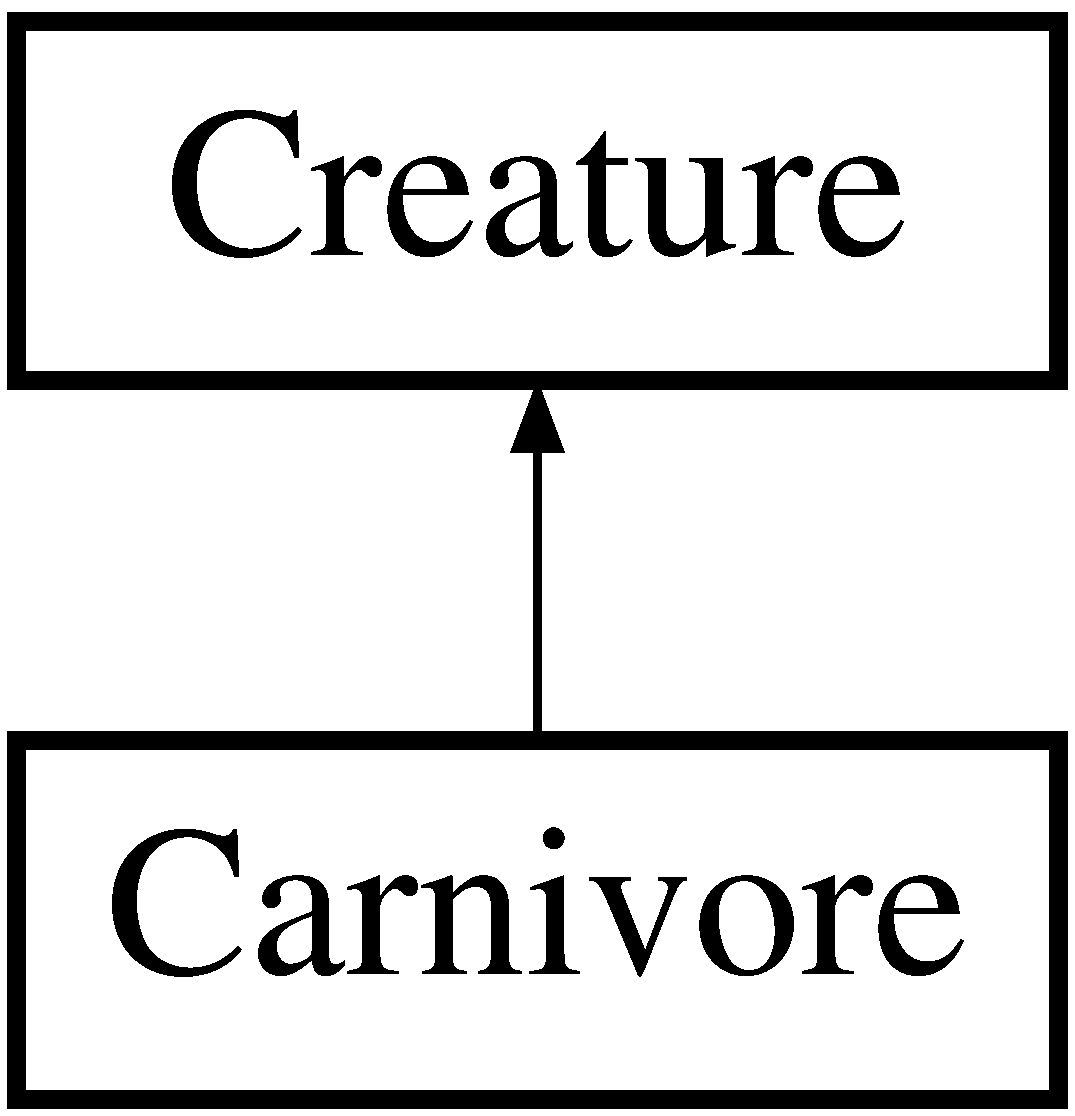
\includegraphics[height=2.000000cm]{class_carnivore}
\end{center}
\end{figure}
\subsection*{Public Member Functions}
\begin{DoxyCompactItemize}
\item 
\mbox{\Hypertarget{class_carnivore_a7ff306fd25d0d26f5e785f80aef202c1}\label{class_carnivore_a7ff306fd25d0d26f5e785f80aef202c1}} 
{\bfseries Carnivore} (\hyperlink{class_creature}{Creature} \&creature)
\item 
\mbox{\Hypertarget{class_carnivore_a2ccf871fe78fdf6537e4bbcdbfde8cca}\label{class_carnivore_a2ccf871fe78fdf6537e4bbcdbfde8cca}} 
bool {\bfseries hunt} (\hyperlink{class_creature}{Creature} \&prey)
\item 
\mbox{\Hypertarget{class_carnivore_a17780e68caf7a472474a68948be97f9d}\label{class_carnivore_a17780e68caf7a472474a68948be97f9d}} 
bool {\bfseries hunt} (\hyperlink{class_herbivore}{Herbivore} prey)
\item 
\mbox{\Hypertarget{class_carnivore_a847b767e22daf1d27b453c12ae504c26}\label{class_carnivore_a847b767e22daf1d27b453c12ae504c26}} 
bool {\bfseries hunt} (\hyperlink{class_omnivore}{Omnivore} prey)
\end{DoxyCompactItemize}
\subsection*{Additional Inherited Members}


The documentation for this class was generated from the following file\+:\begin{DoxyCompactItemize}
\item 
carnivore.\+h\end{DoxyCompactItemize}

\hypertarget{structc_coords}{}\section{c\+Coords Struct Reference}
\label{structc_coords}\index{c\+Coords@{c\+Coords}}
\subsection*{Public Attributes}
\begin{DoxyCompactItemize}
\item 
\mbox{\Hypertarget{structc_coords_ad59aec6dd9d3383c46818ee646392e64}\label{structc_coords_ad59aec6dd9d3383c46818ee646392e64}} 
string {\bfseries species}
\item 
\mbox{\Hypertarget{structc_coords_add7f64f8db39b7cb7ee4113024d4095b}\label{structc_coords_add7f64f8db39b7cb7ee4113024d4095b}} 
int {\bfseries creature}
\item 
\mbox{\Hypertarget{structc_coords_aee8bc762eddc2b02bce322e34a3b27db}\label{structc_coords_aee8bc762eddc2b02bce322e34a3b27db}} 
bool {\bfseries alive} = true
\end{DoxyCompactItemize}


The documentation for this struct was generated from the following file\+:\begin{DoxyCompactItemize}
\item 
mainwindow.\+cpp\end{DoxyCompactItemize}

\hypertarget{struct_main_window_1_1c_coords}{}\section{Main\+Window\+:\+:c\+Coords Struct Reference}
\label{struct_main_window_1_1c_coords}\index{Main\+Window\+::c\+Coords@{Main\+Window\+::c\+Coords}}
\subsection*{Public Attributes}
\begin{DoxyCompactItemize}
\item 
\mbox{\Hypertarget{struct_main_window_1_1c_coords_aa1dd48a05150578d260c9b8e66d6ef40}\label{struct_main_window_1_1c_coords_aa1dd48a05150578d260c9b8e66d6ef40}} 
string {\bfseries species}
\item 
\mbox{\Hypertarget{struct_main_window_1_1c_coords_ab1c75602ae902c641a3b5a17574d1ede}\label{struct_main_window_1_1c_coords_ab1c75602ae902c641a3b5a17574d1ede}} 
int {\bfseries creature}
\item 
\mbox{\Hypertarget{struct_main_window_1_1c_coords_a916584d859f0b4b674933aa438497599}\label{struct_main_window_1_1c_coords_a916584d859f0b4b674933aa438497599}} 
bool {\bfseries alive} = true
\end{DoxyCompactItemize}


The documentation for this struct was generated from the following file\+:\begin{DoxyCompactItemize}
\item 
mainwindow.\+h\end{DoxyCompactItemize}

\hypertarget{structc_count}{}\section{c\+Count Struct Reference}
\label{structc_count}\index{c\+Count@{c\+Count}}
\subsection*{Public Attributes}
\begin{DoxyCompactItemize}
\item 
\mbox{\Hypertarget{structc_count_af46e3a4ba49475372b75648d783eadd4}\label{structc_count_af46e3a4ba49475372b75648d783eadd4}} 
string {\bfseries species}
\item 
\mbox{\Hypertarget{structc_count_a698745ae3c9758015a887cc57b641643}\label{structc_count_a698745ae3c9758015a887cc57b641643}} 
int {\bfseries count}
\end{DoxyCompactItemize}


The documentation for this struct was generated from the following file\+:\begin{DoxyCompactItemize}
\item 
mainwindow.\+cpp\end{DoxyCompactItemize}

\hypertarget{struct_main_window_1_1c_count}{}\section{Main\+Window\+:\+:c\+Count Struct Reference}
\label{struct_main_window_1_1c_count}\index{Main\+Window\+::c\+Count@{Main\+Window\+::c\+Count}}
\subsection*{Public Attributes}
\begin{DoxyCompactItemize}
\item 
\mbox{\Hypertarget{struct_main_window_1_1c_count_a3a27b9c45544b1b756ef21e9d185b003}\label{struct_main_window_1_1c_count_a3a27b9c45544b1b756ef21e9d185b003}} 
string {\bfseries species}
\item 
\mbox{\Hypertarget{struct_main_window_1_1c_count_abc47f2450f6d9f23e4f74e35d72cc473}\label{struct_main_window_1_1c_count_abc47f2450f6d9f23e4f74e35d72cc473}} 
int {\bfseries count}
\end{DoxyCompactItemize}


The documentation for this struct was generated from the following file\+:\begin{DoxyCompactItemize}
\item 
mainwindow.\+h\end{DoxyCompactItemize}

\hypertarget{class_creature}{}\section{Creature Class Reference}
\label{class_creature}\index{Creature@{Creature}}
Inheritance diagram for Creature\+:\begin{figure}[H]
\begin{center}
\leavevmode
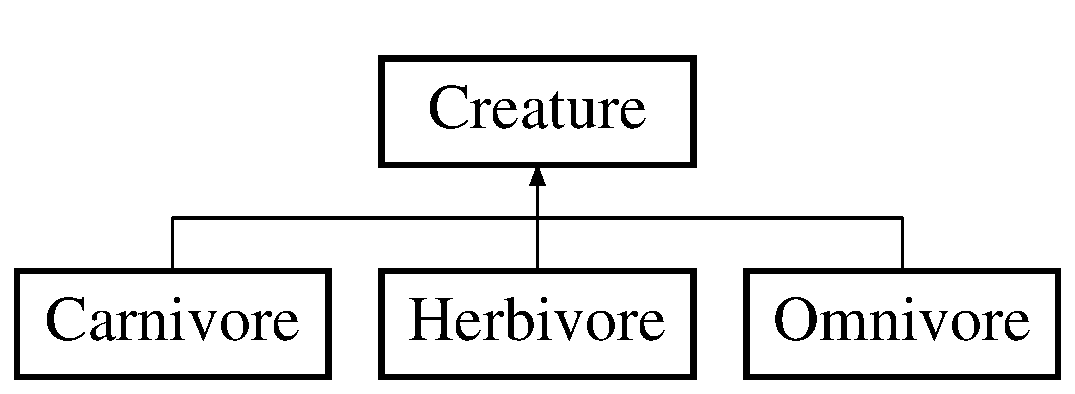
\includegraphics[height=2.000000cm]{class_creature}
\end{center}
\end{figure}
\subsection*{Public Member Functions}
\begin{DoxyCompactItemize}
\item 
\hyperlink{class_creature_a597cc3b08ee17de46c3e7ec3cf0d9b58}{Creature} ()
\item 
virtual \hyperlink{class_creature_aa991b23f4813fbdb6f875204ed49814d}{$\sim$\+Creature} ()
\item 
\hyperlink{class_trait}{Trait} \hyperlink{class_creature_a5cbb05e4ed97cefab203ce1d0a639663}{get\+Trait} (int)
\item 
void \hyperlink{class_creature_a5e9314c792471d371c9255567c7f57f6}{set\+Trait} (int, \hyperlink{class_trait}{Trait})
\item 
void \hyperlink{class_creature_a68390ce1e3db845b569edbb56d2a2e45}{remove\+Trait} (int)
\item 
float \hyperlink{class_creature_aaa5ecf02e6ec776831d68ee031c3a71a}{get\+Age} ()
\item 
void \hyperlink{class_creature_a53a6ce1c089f66f5d72d383918ac6c56}{set\+Age} (float)
\item 
float \hyperlink{class_creature_afbda0cd7841915f1fb1f0b00002e4d9a}{get\+Health} ()
\item 
void \hyperlink{class_creature_a470452d2a72844d841475e2fa1411b87}{set\+Health} (float)
\item 
string \hyperlink{class_creature_a29c472b8d8c500ed750028d35008b874}{get\+Species} ()
\item 
void \hyperlink{class_creature_abe278d213726a2385c03348e0b70baaf}{update\+Health} (float)
\item 
void \hyperlink{class_creature_ad55d859cd054fb78c7ec368a8f93fdab}{set\+Species} ()
\item 
bool \hyperlink{class_creature_a9758254f86daca23432c2aa52388b371}{get\+Diseased} ()
\item 
void \hyperlink{class_creature_a87418faed3520d70b5e79454c51d9d6b}{set\+Diseased} (bool)
\item 
float \hyperlink{class_creature_afc61264e8b9d6e683aa73e225d9165ec}{get\+Water\+Need} ()
\item 
float \hyperlink{class_creature_afaa5a16d665af1b106ea974314ed000b}{get\+Breed\+Chance} (\hyperlink{class_environment}{Environment} Env)
\item 
float \hyperlink{class_creature_a1683c23a3644294d16529feb3d10e2c3}{get\+Herd\+Tendency} ()
\item 
float \hyperlink{class_creature_af2d9ed47b9f8c4baebf8be7f1a6c7c16}{get\+Temp\+Resist} ()
\item 
float \hyperlink{class_creature_a26cacf88614142bfab05c2602088f1ba}{get\+Disease\+Resist} ()
\item 
float \hyperlink{class_creature_af18fa6015052120359c99cd56620c91e}{get\+Predator\+Resist} ()
\item 
void \hyperlink{class_creature_a61b42a4c3fe592a559ccfcef5089d676}{set\+Water\+Need} (float)
\item 
void \hyperlink{class_creature_aa0c973f2abb3cfad7c828b62baf80a33}{set\+Breed\+Chance} (float)
\item 
void \hyperlink{class_creature_ac54280109cd668ca679189c83cf9318c}{set\+Herd\+Tendency} (float)
\item 
void \hyperlink{class_creature_a7e34bf01307d2818cf51f184237a62b8}{set\+Temp\+Resist} (float)
\item 
void \hyperlink{class_creature_a76623b331f8a5051c8ab6aa122ed3091}{set\+Diease\+Resist} (float)
\item 
void \hyperlink{class_creature_a1e8c730feef5947ead25549f7b43c36c}{set\+Predator\+Resist} (float)
\item 
bool \hyperlink{class_creature_a3316556d75305448ffb28a26d7eaa0ad}{update\+Health} (\hyperlink{class_environment}{Environment} \&)
\item 
void \hyperlink{class_creature_a87624b71be563323455cb5241aba25b4}{calc\+Stats} (\hyperlink{class_environment}{Environment})
\item 
\hyperlink{class_creature}{Creature} \hyperlink{class_creature_aa3495553c53d7743c158d961827ec81f}{breed} (\hyperlink{class_creature}{Creature}, int)
\item 
string \hyperlink{class_creature_a22ba2327e33a9e8554284f485ad9cf0f}{to\+String} ()
\end{DoxyCompactItemize}
\subsection*{Public Attributes}
\begin{DoxyCompactItemize}
\item 
\mbox{\Hypertarget{class_creature_adab2dc50d1556d82299c3dd3db9597f8}\label{class_creature_adab2dc50d1556d82299c3dd3db9597f8}} 
int {\bfseries index}
\end{DoxyCompactItemize}
\subsection*{Protected Attributes}
\begin{DoxyCompactItemize}
\item 
\mbox{\Hypertarget{class_creature_a4240e372407b7df5614b0766f95524a8}\label{class_creature_a4240e372407b7df5614b0766f95524a8}} 
float {\bfseries water\+Need}
\item 
\mbox{\Hypertarget{class_creature_a66cb1f9c65d6b63976b00e03c9174868}\label{class_creature_a66cb1f9c65d6b63976b00e03c9174868}} 
float {\bfseries breed\+Chance}
\item 
\mbox{\Hypertarget{class_creature_aeac241536d909e12cbae19d1577a8cbe}\label{class_creature_aeac241536d909e12cbae19d1577a8cbe}} 
float {\bfseries herd\+Tendency}
\item 
\mbox{\Hypertarget{class_creature_a53c8032f68153df41f7b22796eb72bd0}\label{class_creature_a53c8032f68153df41f7b22796eb72bd0}} 
float {\bfseries temp\+\_\+resist}
\item 
\mbox{\Hypertarget{class_creature_a797fc79828501798cd216f56471583fc}\label{class_creature_a797fc79828501798cd216f56471583fc}} 
float {\bfseries disease\+\_\+resist}
\item 
\mbox{\Hypertarget{class_creature_a85bd79783c5a8f9b0de2c7be338d0eca}\label{class_creature_a85bd79783c5a8f9b0de2c7be338d0eca}} 
float {\bfseries predator\+\_\+resist}
\end{DoxyCompactItemize}


\subsection{Constructor \& Destructor Documentation}
\mbox{\Hypertarget{class_creature_a597cc3b08ee17de46c3e7ec3cf0d9b58}\label{class_creature_a597cc3b08ee17de46c3e7ec3cf0d9b58}} 
\index{Creature@{Creature}!Creature@{Creature}}
\index{Creature@{Creature}!Creature@{Creature}}
\subsubsection{\texorpdfstring{Creature()}{Creature()}}
{\footnotesize\ttfamily Creature\+::\+Creature (\begin{DoxyParamCaption}{ }\end{DoxyParamCaption})}

Default Constructor. Sets default values for \hyperlink{class_creature}{Creature} class. 
\begin{DoxyParams}{Parameters}
{\em none} & \\
\hline
\end{DoxyParams}
\mbox{\Hypertarget{class_creature_aa991b23f4813fbdb6f875204ed49814d}\label{class_creature_aa991b23f4813fbdb6f875204ed49814d}} 
\index{Creature@{Creature}!````~Creature@{$\sim$\+Creature}}
\index{````~Creature@{$\sim$\+Creature}!Creature@{Creature}}
\subsubsection{\texorpdfstring{$\sim$\+Creature()}{~Creature()}}
{\footnotesize\ttfamily Creature\+::$\sim$\+Creature (\begin{DoxyParamCaption}{ }\end{DoxyParamCaption})\hspace{0.3cm}{\ttfamily [virtual]}}

Destructor for \hyperlink{class_creature}{Creature}. 
\begin{DoxyParams}{Parameters}
{\em none} & \\
\hline
\end{DoxyParams}


\subsection{Member Function Documentation}
\mbox{\Hypertarget{class_creature_aa3495553c53d7743c158d961827ec81f}\label{class_creature_aa3495553c53d7743c158d961827ec81f}} 
\index{Creature@{Creature}!breed@{breed}}
\index{breed@{breed}!Creature@{Creature}}
\subsubsection{\texorpdfstring{breed()}{breed()}}
{\footnotesize\ttfamily \hyperlink{class_creature}{Creature} Creature\+::breed (\begin{DoxyParamCaption}\item[{\hyperlink{class_creature}{Creature}}]{other,  }\item[{int}]{breed }\end{DoxyParamCaption})}

Method. Allows a \hyperlink{class_creature}{Creature} to breed. 
\begin{DoxyParams}{Parameters}
{\em other} & \\
\hline
{\em breed} & \\
\hline
\end{DoxyParams}
\begin{DoxyReturn}{Returns}
baby 
\end{DoxyReturn}
\mbox{\Hypertarget{class_creature_a87624b71be563323455cb5241aba25b4}\label{class_creature_a87624b71be563323455cb5241aba25b4}} 
\index{Creature@{Creature}!calc\+Stats@{calc\+Stats}}
\index{calc\+Stats@{calc\+Stats}!Creature@{Creature}}
\subsubsection{\texorpdfstring{calc\+Stats()}{calcStats()}}
{\footnotesize\ttfamily void Creature\+::calc\+Stats (\begin{DoxyParamCaption}\item[{\hyperlink{class_environment}{Environment}}]{Env }\end{DoxyParamCaption})}

Method. Calculates the statistics for a \hyperlink{class_creature}{Creature}. 
\begin{DoxyParams}{Parameters}
{\em Env} & \\
\hline
\end{DoxyParams}
\begin{DoxyReturn}{Returns}
none 
\end{DoxyReturn}
\mbox{\Hypertarget{class_creature_aaa5ecf02e6ec776831d68ee031c3a71a}\label{class_creature_aaa5ecf02e6ec776831d68ee031c3a71a}} 
\index{Creature@{Creature}!get\+Age@{get\+Age}}
\index{get\+Age@{get\+Age}!Creature@{Creature}}
\subsubsection{\texorpdfstring{get\+Age()}{getAge()}}
{\footnotesize\ttfamily float Creature\+::get\+Age (\begin{DoxyParamCaption}{ }\end{DoxyParamCaption})}

Getter. Returns \hyperlink{class_creature}{Creature}\textquotesingle{}s age. 
\begin{DoxyParams}{Parameters}
{\em none} & \\
\hline
\end{DoxyParams}
\begin{DoxyReturn}{Returns}
age 
\end{DoxyReturn}
\mbox{\Hypertarget{class_creature_afaa5a16d665af1b106ea974314ed000b}\label{class_creature_afaa5a16d665af1b106ea974314ed000b}} 
\index{Creature@{Creature}!get\+Breed\+Chance@{get\+Breed\+Chance}}
\index{get\+Breed\+Chance@{get\+Breed\+Chance}!Creature@{Creature}}
\subsubsection{\texorpdfstring{get\+Breed\+Chance()}{getBreedChance()}}
{\footnotesize\ttfamily float Creature\+::get\+Breed\+Chance (\begin{DoxyParamCaption}\item[{\hyperlink{class_environment}{Environment}}]{Env }\end{DoxyParamCaption})}

Getter. Returns breed chance of a \hyperlink{class_creature}{Creature}. 
\begin{DoxyParams}{Parameters}
{\em Env} & \\
\hline
\end{DoxyParams}
\begin{DoxyReturn}{Returns}
breed\+Chance 
\end{DoxyReturn}
\mbox{\Hypertarget{class_creature_a9758254f86daca23432c2aa52388b371}\label{class_creature_a9758254f86daca23432c2aa52388b371}} 
\index{Creature@{Creature}!get\+Diseased@{get\+Diseased}}
\index{get\+Diseased@{get\+Diseased}!Creature@{Creature}}
\subsubsection{\texorpdfstring{get\+Diseased()}{getDiseased()}}
{\footnotesize\ttfamily bool Creature\+::get\+Diseased (\begin{DoxyParamCaption}{ }\end{DoxyParamCaption})}

Getter. Gets bool value representing whether or not a creature is diseased. 
\begin{DoxyParams}{Parameters}
{\em none} & \\
\hline
\end{DoxyParams}
\begin{DoxyReturn}{Returns}
diseased 
\end{DoxyReturn}
\mbox{\Hypertarget{class_creature_a26cacf88614142bfab05c2602088f1ba}\label{class_creature_a26cacf88614142bfab05c2602088f1ba}} 
\index{Creature@{Creature}!get\+Disease\+Resist@{get\+Disease\+Resist}}
\index{get\+Disease\+Resist@{get\+Disease\+Resist}!Creature@{Creature}}
\subsubsection{\texorpdfstring{get\+Disease\+Resist()}{getDiseaseResist()}}
{\footnotesize\ttfamily float Creature\+::get\+Disease\+Resist (\begin{DoxyParamCaption}{ }\end{DoxyParamCaption})}

Getter. Returns disease resistance of a \hyperlink{class_creature}{Creature}. 
\begin{DoxyParams}{Parameters}
{\em none} & \\
\hline
\end{DoxyParams}
\begin{DoxyReturn}{Returns}
disease\+\_\+resist 
\end{DoxyReturn}
\mbox{\Hypertarget{class_creature_afbda0cd7841915f1fb1f0b00002e4d9a}\label{class_creature_afbda0cd7841915f1fb1f0b00002e4d9a}} 
\index{Creature@{Creature}!get\+Health@{get\+Health}}
\index{get\+Health@{get\+Health}!Creature@{Creature}}
\subsubsection{\texorpdfstring{get\+Health()}{getHealth()}}
{\footnotesize\ttfamily float Creature\+::get\+Health (\begin{DoxyParamCaption}{ }\end{DoxyParamCaption})}

Getter. Gets \hyperlink{class_creature}{Creature}\textquotesingle{}s health. 
\begin{DoxyParams}{Parameters}
{\em none} & \\
\hline
\end{DoxyParams}
\begin{DoxyReturn}{Returns}
health 
\end{DoxyReturn}
\mbox{\Hypertarget{class_creature_a1683c23a3644294d16529feb3d10e2c3}\label{class_creature_a1683c23a3644294d16529feb3d10e2c3}} 
\index{Creature@{Creature}!get\+Herd\+Tendency@{get\+Herd\+Tendency}}
\index{get\+Herd\+Tendency@{get\+Herd\+Tendency}!Creature@{Creature}}
\subsubsection{\texorpdfstring{get\+Herd\+Tendency()}{getHerdTendency()}}
{\footnotesize\ttfamily float Creature\+::get\+Herd\+Tendency (\begin{DoxyParamCaption}{ }\end{DoxyParamCaption})}

Getter. Returns herd tendency of a \hyperlink{class_creature}{Creature}. 
\begin{DoxyParams}{Parameters}
{\em none} & \\
\hline
\end{DoxyParams}
\begin{DoxyReturn}{Returns}
herd\+Tendency 
\end{DoxyReturn}
\mbox{\Hypertarget{class_creature_af18fa6015052120359c99cd56620c91e}\label{class_creature_af18fa6015052120359c99cd56620c91e}} 
\index{Creature@{Creature}!get\+Predator\+Resist@{get\+Predator\+Resist}}
\index{get\+Predator\+Resist@{get\+Predator\+Resist}!Creature@{Creature}}
\subsubsection{\texorpdfstring{get\+Predator\+Resist()}{getPredatorResist()}}
{\footnotesize\ttfamily float Creature\+::get\+Predator\+Resist (\begin{DoxyParamCaption}{ }\end{DoxyParamCaption})}

Getter. Returns predator resistance of a \hyperlink{class_creature}{Creature}. 
\begin{DoxyParams}{Parameters}
{\em none} & \\
\hline
\end{DoxyParams}
\begin{DoxyReturn}{Returns}
predator\+\_\+resist 
\end{DoxyReturn}
\mbox{\Hypertarget{class_creature_a29c472b8d8c500ed750028d35008b874}\label{class_creature_a29c472b8d8c500ed750028d35008b874}} 
\index{Creature@{Creature}!get\+Species@{get\+Species}}
\index{get\+Species@{get\+Species}!Creature@{Creature}}
\subsubsection{\texorpdfstring{get\+Species()}{getSpecies()}}
{\footnotesize\ttfamily string Creature\+::get\+Species (\begin{DoxyParamCaption}{ }\end{DoxyParamCaption})}

Getter. Gets \hyperlink{class_creature}{Creature}\textquotesingle{}s Species. 
\begin{DoxyParams}{Parameters}
{\em none} & \\
\hline
\end{DoxyParams}
\begin{DoxyReturn}{Returns}
species 
\end{DoxyReturn}
\mbox{\Hypertarget{class_creature_af2d9ed47b9f8c4baebf8be7f1a6c7c16}\label{class_creature_af2d9ed47b9f8c4baebf8be7f1a6c7c16}} 
\index{Creature@{Creature}!get\+Temp\+Resist@{get\+Temp\+Resist}}
\index{get\+Temp\+Resist@{get\+Temp\+Resist}!Creature@{Creature}}
\subsubsection{\texorpdfstring{get\+Temp\+Resist()}{getTempResist()}}
{\footnotesize\ttfamily float Creature\+::get\+Temp\+Resist (\begin{DoxyParamCaption}{ }\end{DoxyParamCaption})}

Getter. Returns temperature resistance of a \hyperlink{class_creature}{Creature}. 
\begin{DoxyParams}{Parameters}
{\em none} & \\
\hline
\end{DoxyParams}
\begin{DoxyReturn}{Returns}
temp\+\_\+resist 
\end{DoxyReturn}
\mbox{\Hypertarget{class_creature_a5cbb05e4ed97cefab203ce1d0a639663}\label{class_creature_a5cbb05e4ed97cefab203ce1d0a639663}} 
\index{Creature@{Creature}!get\+Trait@{get\+Trait}}
\index{get\+Trait@{get\+Trait}!Creature@{Creature}}
\subsubsection{\texorpdfstring{get\+Trait()}{getTrait()}}
{\footnotesize\ttfamily \hyperlink{class_trait}{Trait} Creature\+::get\+Trait (\begin{DoxyParamCaption}\item[{int}]{index }\end{DoxyParamCaption})}

Getter. Gets each \hyperlink{class_trait}{Trait} for a \hyperlink{class_creature}{Creature}. 
\begin{DoxyParams}{Parameters}
{\em index} & \\
\hline
\end{DoxyParams}
\begin{DoxyReturn}{Returns}
traits\mbox{[}index\mbox{]} 
\end{DoxyReturn}
\mbox{\Hypertarget{class_creature_afc61264e8b9d6e683aa73e225d9165ec}\label{class_creature_afc61264e8b9d6e683aa73e225d9165ec}} 
\index{Creature@{Creature}!get\+Water\+Need@{get\+Water\+Need}}
\index{get\+Water\+Need@{get\+Water\+Need}!Creature@{Creature}}
\subsubsection{\texorpdfstring{get\+Water\+Need()}{getWaterNeed()}}
{\footnotesize\ttfamily float Creature\+::get\+Water\+Need (\begin{DoxyParamCaption}{ }\end{DoxyParamCaption})}

Getter. Returns water need for a \hyperlink{class_creature}{Creature}. 
\begin{DoxyParams}{Parameters}
{\em none} & \\
\hline
\end{DoxyParams}
\begin{DoxyReturn}{Returns}
water\+Need 
\end{DoxyReturn}
\mbox{\Hypertarget{class_creature_a68390ce1e3db845b569edbb56d2a2e45}\label{class_creature_a68390ce1e3db845b569edbb56d2a2e45}} 
\index{Creature@{Creature}!remove\+Trait@{remove\+Trait}}
\index{remove\+Trait@{remove\+Trait}!Creature@{Creature}}
\subsubsection{\texorpdfstring{remove\+Trait()}{removeTrait()}}
{\footnotesize\ttfamily void Creature\+::remove\+Trait (\begin{DoxyParamCaption}\item[{int}]{index }\end{DoxyParamCaption})}

Method. Removes \hyperlink{class_trait}{Trait} for a \hyperlink{class_creature}{Creature}. 
\begin{DoxyParams}{Parameters}
{\em index} & \\
\hline
\end{DoxyParams}
\begin{DoxyReturn}{Returns}
none 
\end{DoxyReturn}
\mbox{\Hypertarget{class_creature_a53a6ce1c089f66f5d72d383918ac6c56}\label{class_creature_a53a6ce1c089f66f5d72d383918ac6c56}} 
\index{Creature@{Creature}!set\+Age@{set\+Age}}
\index{set\+Age@{set\+Age}!Creature@{Creature}}
\subsubsection{\texorpdfstring{set\+Age()}{setAge()}}
{\footnotesize\ttfamily void Creature\+::set\+Age (\begin{DoxyParamCaption}\item[{float}]{n\+Age }\end{DoxyParamCaption})}

Setter. Sets \hyperlink{class_creature}{Creature}\textquotesingle{}s age. 
\begin{DoxyParams}{Parameters}
{\em n\+Age} & \\
\hline
\end{DoxyParams}
\begin{DoxyReturn}{Returns}
none 
\end{DoxyReturn}
\mbox{\Hypertarget{class_creature_aa0c973f2abb3cfad7c828b62baf80a33}\label{class_creature_aa0c973f2abb3cfad7c828b62baf80a33}} 
\index{Creature@{Creature}!set\+Breed\+Chance@{set\+Breed\+Chance}}
\index{set\+Breed\+Chance@{set\+Breed\+Chance}!Creature@{Creature}}
\subsubsection{\texorpdfstring{set\+Breed\+Chance()}{setBreedChance()}}
{\footnotesize\ttfamily void Creature\+::set\+Breed\+Chance (\begin{DoxyParamCaption}\item[{float}]{bc }\end{DoxyParamCaption})}

Setter. Sets a \hyperlink{class_creature}{Creature}\textquotesingle{}s breed chance. 
\begin{DoxyParams}{Parameters}
{\em bc} & \\
\hline
\end{DoxyParams}
\begin{DoxyReturn}{Returns}
none 
\end{DoxyReturn}
\mbox{\Hypertarget{class_creature_a76623b331f8a5051c8ab6aa122ed3091}\label{class_creature_a76623b331f8a5051c8ab6aa122ed3091}} 
\index{Creature@{Creature}!set\+Diease\+Resist@{set\+Diease\+Resist}}
\index{set\+Diease\+Resist@{set\+Diease\+Resist}!Creature@{Creature}}
\subsubsection{\texorpdfstring{set\+Diease\+Resist()}{setDieaseResist()}}
{\footnotesize\ttfamily void Creature\+::set\+Diease\+Resist (\begin{DoxyParamCaption}\item[{float}]{dr }\end{DoxyParamCaption})}

Setter. Setss a \hyperlink{class_creature}{Creature}\textquotesingle{}s disease resistance. 
\begin{DoxyParams}{Parameters}
{\em dr} & \\
\hline
\end{DoxyParams}
\begin{DoxyReturn}{Returns}
none 
\end{DoxyReturn}
\mbox{\Hypertarget{class_creature_a87418faed3520d70b5e79454c51d9d6b}\label{class_creature_a87418faed3520d70b5e79454c51d9d6b}} 
\index{Creature@{Creature}!set\+Diseased@{set\+Diseased}}
\index{set\+Diseased@{set\+Diseased}!Creature@{Creature}}
\subsubsection{\texorpdfstring{set\+Diseased()}{setDiseased()}}
{\footnotesize\ttfamily void Creature\+::set\+Diseased (\begin{DoxyParamCaption}\item[{bool}]{dis }\end{DoxyParamCaption})}

Setter. Sets diseased value to a true/false input value. 
\begin{DoxyParams}{Parameters}
{\em dis} & \\
\hline
\end{DoxyParams}
\begin{DoxyReturn}{Returns}
none 
\end{DoxyReturn}
\mbox{\Hypertarget{class_creature_a470452d2a72844d841475e2fa1411b87}\label{class_creature_a470452d2a72844d841475e2fa1411b87}} 
\index{Creature@{Creature}!set\+Health@{set\+Health}}
\index{set\+Health@{set\+Health}!Creature@{Creature}}
\subsubsection{\texorpdfstring{set\+Health()}{setHealth()}}
{\footnotesize\ttfamily void Creature\+::set\+Health (\begin{DoxyParamCaption}\item[{float}]{n\+Health }\end{DoxyParamCaption})}

Setter. Sets \hyperlink{class_creature}{Creature}\textquotesingle{}s health. 
\begin{DoxyParams}{Parameters}
{\em n\+Health} & \\
\hline
\end{DoxyParams}
\begin{DoxyReturn}{Returns}
none 
\end{DoxyReturn}
\mbox{\Hypertarget{class_creature_ac54280109cd668ca679189c83cf9318c}\label{class_creature_ac54280109cd668ca679189c83cf9318c}} 
\index{Creature@{Creature}!set\+Herd\+Tendency@{set\+Herd\+Tendency}}
\index{set\+Herd\+Tendency@{set\+Herd\+Tendency}!Creature@{Creature}}
\subsubsection{\texorpdfstring{set\+Herd\+Tendency()}{setHerdTendency()}}
{\footnotesize\ttfamily void Creature\+::set\+Herd\+Tendency (\begin{DoxyParamCaption}\item[{float}]{ht }\end{DoxyParamCaption})}

Setter. Sets a \hyperlink{class_creature}{Creature}\textquotesingle{}s herd tendency. 
\begin{DoxyParams}{Parameters}
{\em ht} & \\
\hline
\end{DoxyParams}
\begin{DoxyReturn}{Returns}
none 
\end{DoxyReturn}
\mbox{\Hypertarget{class_creature_a1e8c730feef5947ead25549f7b43c36c}\label{class_creature_a1e8c730feef5947ead25549f7b43c36c}} 
\index{Creature@{Creature}!set\+Predator\+Resist@{set\+Predator\+Resist}}
\index{set\+Predator\+Resist@{set\+Predator\+Resist}!Creature@{Creature}}
\subsubsection{\texorpdfstring{set\+Predator\+Resist()}{setPredatorResist()}}
{\footnotesize\ttfamily void Creature\+::set\+Predator\+Resist (\begin{DoxyParamCaption}\item[{float}]{pr }\end{DoxyParamCaption})}

Setter. Sets a \hyperlink{class_creature}{Creature}\textquotesingle{}s predator resistance. 
\begin{DoxyParams}{Parameters}
{\em pr} & \\
\hline
\end{DoxyParams}
\begin{DoxyReturn}{Returns}
none 
\end{DoxyReturn}
\mbox{\Hypertarget{class_creature_ad55d859cd054fb78c7ec368a8f93fdab}\label{class_creature_ad55d859cd054fb78c7ec368a8f93fdab}} 
\index{Creature@{Creature}!set\+Species@{set\+Species}}
\index{set\+Species@{set\+Species}!Creature@{Creature}}
\subsubsection{\texorpdfstring{set\+Species()}{setSpecies()}}
{\footnotesize\ttfamily void Creature\+::set\+Species (\begin{DoxyParamCaption}{ }\end{DoxyParamCaption})}

Method. Determines name for a species. 
\begin{DoxyParams}{Parameters}
{\em none} & \\
\hline
\end{DoxyParams}
\begin{DoxyReturn}{Returns}
none 
\end{DoxyReturn}
\mbox{\Hypertarget{class_creature_a7e34bf01307d2818cf51f184237a62b8}\label{class_creature_a7e34bf01307d2818cf51f184237a62b8}} 
\index{Creature@{Creature}!set\+Temp\+Resist@{set\+Temp\+Resist}}
\index{set\+Temp\+Resist@{set\+Temp\+Resist}!Creature@{Creature}}
\subsubsection{\texorpdfstring{set\+Temp\+Resist()}{setTempResist()}}
{\footnotesize\ttfamily void Creature\+::set\+Temp\+Resist (\begin{DoxyParamCaption}\item[{float}]{tr }\end{DoxyParamCaption})}

Setter. Sets a \hyperlink{class_creature}{Creature}\textquotesingle{}s temperature resistance. 
\begin{DoxyParams}{Parameters}
{\em tr} & \\
\hline
\end{DoxyParams}
\begin{DoxyReturn}{Returns}
none 
\end{DoxyReturn}
\mbox{\Hypertarget{class_creature_a5e9314c792471d371c9255567c7f57f6}\label{class_creature_a5e9314c792471d371c9255567c7f57f6}} 
\index{Creature@{Creature}!set\+Trait@{set\+Trait}}
\index{set\+Trait@{set\+Trait}!Creature@{Creature}}
\subsubsection{\texorpdfstring{set\+Trait()}{setTrait()}}
{\footnotesize\ttfamily void Creature\+::set\+Trait (\begin{DoxyParamCaption}\item[{int}]{index,  }\item[{\hyperlink{class_trait}{Trait}}]{new\+Trait }\end{DoxyParamCaption})}

Setter. Sets \hyperlink{class_trait}{Trait} at index value for a \hyperlink{class_creature}{Creature}. 
\begin{DoxyParams}{Parameters}
{\em index} & \\
\hline
{\em new\+Trait} & \\
\hline
\end{DoxyParams}
\begin{DoxyReturn}{Returns}
none 
\end{DoxyReturn}
\mbox{\Hypertarget{class_creature_a61b42a4c3fe592a559ccfcef5089d676}\label{class_creature_a61b42a4c3fe592a559ccfcef5089d676}} 
\index{Creature@{Creature}!set\+Water\+Need@{set\+Water\+Need}}
\index{set\+Water\+Need@{set\+Water\+Need}!Creature@{Creature}}
\subsubsection{\texorpdfstring{set\+Water\+Need()}{setWaterNeed()}}
{\footnotesize\ttfamily void Creature\+::set\+Water\+Need (\begin{DoxyParamCaption}\item[{float}]{wn }\end{DoxyParamCaption})}

Setter. Sets water need for a \hyperlink{class_creature}{Creature}. 
\begin{DoxyParams}{Parameters}
{\em wn} & \\
\hline
\end{DoxyParams}
\begin{DoxyReturn}{Returns}
none 
\end{DoxyReturn}
\mbox{\Hypertarget{class_creature_a22ba2327e33a9e8554284f485ad9cf0f}\label{class_creature_a22ba2327e33a9e8554284f485ad9cf0f}} 
\index{Creature@{Creature}!to\+String@{to\+String}}
\index{to\+String@{to\+String}!Creature@{Creature}}
\subsubsection{\texorpdfstring{to\+String()}{toString()}}
{\footnotesize\ttfamily string Creature\+::to\+String (\begin{DoxyParamCaption}{ }\end{DoxyParamCaption})}

Method. To\+String for \hyperlink{class_creature}{Creature} class. 
\begin{DoxyParams}{Parameters}
{\em none} & \\
\hline
\end{DoxyParams}
\begin{DoxyReturn}{Returns}
c\+String 
\end{DoxyReturn}
\mbox{\Hypertarget{class_creature_abe278d213726a2385c03348e0b70baaf}\label{class_creature_abe278d213726a2385c03348e0b70baaf}} 
\index{Creature@{Creature}!update\+Health@{update\+Health}}
\index{update\+Health@{update\+Health}!Creature@{Creature}}
\subsubsection{\texorpdfstring{update\+Health()}{updateHealth()}\hspace{0.1cm}{\footnotesize\ttfamily [1/2]}}
{\footnotesize\ttfamily void Creature\+::update\+Health (\begin{DoxyParamCaption}\item[{float}]{update }\end{DoxyParamCaption})}

Method. Updates \hyperlink{class_creature}{Creature}\textquotesingle{}s health. 
\begin{DoxyParams}{Parameters}
{\em update} & \\
\hline
\end{DoxyParams}
\begin{DoxyReturn}{Returns}
none 
\end{DoxyReturn}
\mbox{\Hypertarget{class_creature_a3316556d75305448ffb28a26d7eaa0ad}\label{class_creature_a3316556d75305448ffb28a26d7eaa0ad}} 
\index{Creature@{Creature}!update\+Health@{update\+Health}}
\index{update\+Health@{update\+Health}!Creature@{Creature}}
\subsubsection{\texorpdfstring{update\+Health()}{updateHealth()}\hspace{0.1cm}{\footnotesize\ttfamily [2/2]}}
{\footnotesize\ttfamily bool Creature\+::update\+Health (\begin{DoxyParamCaption}\item[{\hyperlink{class_environment}{Environment} \&}]{Env }\end{DoxyParamCaption})}

Method. Updates a \hyperlink{class_creature}{Creature}\textquotesingle{}s health 
\begin{DoxyParams}{Parameters}
{\em Env} & \\
\hline
\end{DoxyParams}
\begin{DoxyReturn}{Returns}
boolean 
\end{DoxyReturn}


The documentation for this class was generated from the following files\+:\begin{DoxyCompactItemize}
\item 
creature.\+h\item 
creature.\+cpp\end{DoxyCompactItemize}

\hypertarget{classdetailwindow}{}\section{detailwindow Class Reference}
\label{classdetailwindow}\index{detailwindow@{detailwindow}}
Inheritance diagram for detailwindow\+:\begin{figure}[H]
\begin{center}
\leavevmode
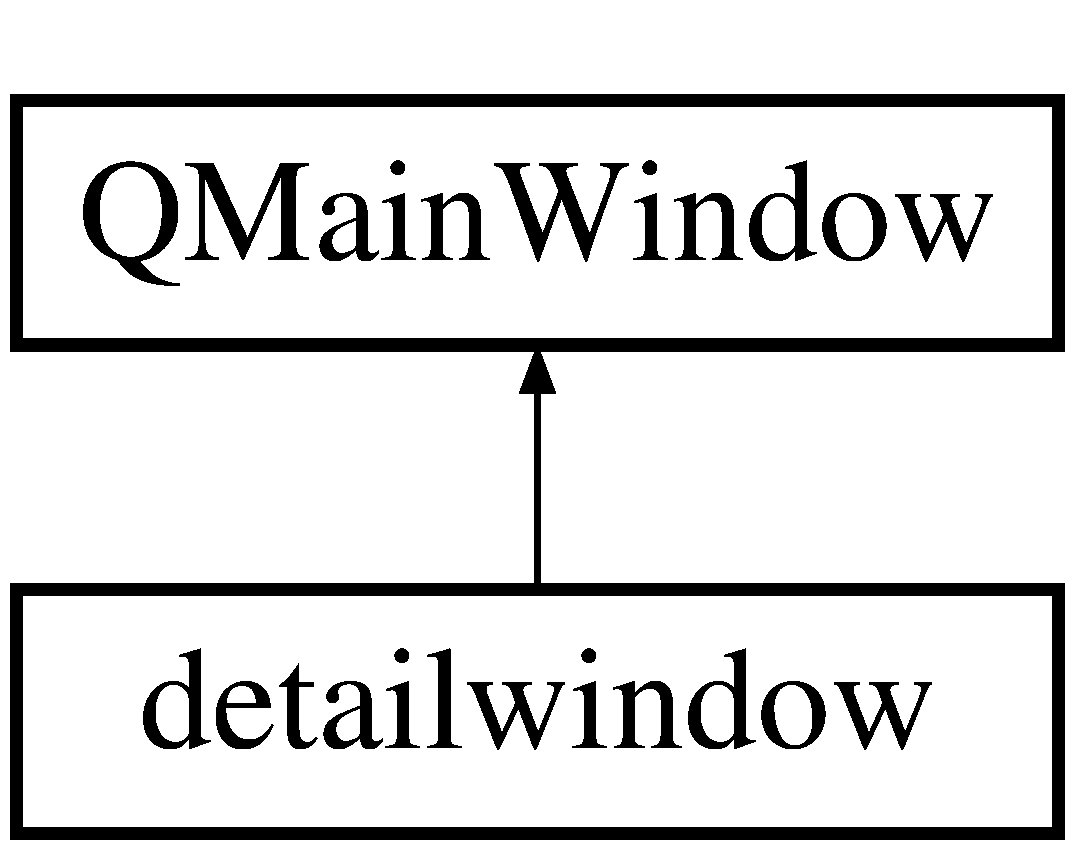
\includegraphics[height=2.000000cm]{classdetailwindow}
\end{center}
\end{figure}
\subsection*{Public Member Functions}
\begin{DoxyCompactItemize}
\item 
\hyperlink{classdetailwindow_abedfe426704c69d9fb1dd01870fdc47b}{detailwindow} (Q\+Widget $\ast$parent=0)
\item 
\hyperlink{classdetailwindow_a4423d1b152631ad2bb6838b3a77f0315}{$\sim$detailwindow} ()
\item 
void \hyperlink{classdetailwindow_adfcea879c00c9905840988e777f809b3}{setcounts} (int, int)
\item 
void \hyperlink{classdetailwindow_acc6d6b4b1ab5141927c6acddf36f43ff}{setcols} (int)
\item 
void \hyperlink{classdetailwindow_a574edec5e903abfe41cf47db896c5f20}{setrows} (int)
\item 
void \hyperlink{classdetailwindow_a961ee64e60bff473f929629f9335518f}{insertrow} (int)
\item 
void \hyperlink{classdetailwindow_ab64a227e7c07e5dc17e7a0a29675544a}{insertitem} (int, int, Q\+Table\+Widget\+Item $\ast$)
\end{DoxyCompactItemize}


\subsection{Constructor \& Destructor Documentation}
\mbox{\Hypertarget{classdetailwindow_abedfe426704c69d9fb1dd01870fdc47b}\label{classdetailwindow_abedfe426704c69d9fb1dd01870fdc47b}} 
\index{detailwindow@{detailwindow}!detailwindow@{detailwindow}}
\index{detailwindow@{detailwindow}!detailwindow@{detailwindow}}
\subsubsection{\texorpdfstring{detailwindow()}{detailwindow()}}
{\footnotesize\ttfamily detailwindow\+::detailwindow (\begin{DoxyParamCaption}\item[{Q\+Widget $\ast$}]{parent = {\ttfamily 0} }\end{DoxyParamCaption})\hspace{0.3cm}{\ttfamily [explicit]}}

Constructor. Sets up Q\+Widget and UI for the Detail\+Window. 
\begin{DoxyParams}{Parameters}
{\em parent} & \\
\hline
\end{DoxyParams}
\begin{DoxyReturn}{Returns}
none 
\end{DoxyReturn}
\mbox{\Hypertarget{classdetailwindow_a4423d1b152631ad2bb6838b3a77f0315}\label{classdetailwindow_a4423d1b152631ad2bb6838b3a77f0315}} 
\index{detailwindow@{detailwindow}!````~detailwindow@{$\sim$detailwindow}}
\index{````~detailwindow@{$\sim$detailwindow}!detailwindow@{detailwindow}}
\subsubsection{\texorpdfstring{$\sim$detailwindow()}{~detailwindow()}}
{\footnotesize\ttfamily detailwindow\+::$\sim$detailwindow (\begin{DoxyParamCaption}{ }\end{DoxyParamCaption})}

Destructor for Detail\+Window. 
\begin{DoxyParams}{Parameters}
{\em none} & \\
\hline
\end{DoxyParams}
\begin{DoxyReturn}{Returns}
none 
\end{DoxyReturn}


\subsection{Member Function Documentation}
\mbox{\Hypertarget{classdetailwindow_ab64a227e7c07e5dc17e7a0a29675544a}\label{classdetailwindow_ab64a227e7c07e5dc17e7a0a29675544a}} 
\index{detailwindow@{detailwindow}!insertitem@{insertitem}}
\index{insertitem@{insertitem}!detailwindow@{detailwindow}}
\subsubsection{\texorpdfstring{insertitem()}{insertitem()}}
{\footnotesize\ttfamily void detailwindow\+::insertitem (\begin{DoxyParamCaption}\item[{int}]{r,  }\item[{int}]{c,  }\item[{Q\+Table\+Widget\+Item $\ast$}]{t }\end{DoxyParamCaption})}

Method. Inserts item into row and column in table. 
\begin{DoxyParams}{Parameters}
{\em r} & \\
\hline
{\em c} & \\
\hline
{\em t} & \\
\hline
\end{DoxyParams}
\begin{DoxyReturn}{Returns}
none 
\end{DoxyReturn}
\mbox{\Hypertarget{classdetailwindow_a961ee64e60bff473f929629f9335518f}\label{classdetailwindow_a961ee64e60bff473f929629f9335518f}} 
\index{detailwindow@{detailwindow}!insertrow@{insertrow}}
\index{insertrow@{insertrow}!detailwindow@{detailwindow}}
\subsubsection{\texorpdfstring{insertrow()}{insertrow()}}
{\footnotesize\ttfamily void detailwindow\+::insertrow (\begin{DoxyParamCaption}\item[{int}]{r }\end{DoxyParamCaption})}

Method. Inserts row into specified spot. 
\begin{DoxyParams}{Parameters}
{\em r} & \\
\hline
\end{DoxyParams}
\begin{DoxyReturn}{Returns}
none 
\end{DoxyReturn}
\mbox{\Hypertarget{classdetailwindow_acc6d6b4b1ab5141927c6acddf36f43ff}\label{classdetailwindow_acc6d6b4b1ab5141927c6acddf36f43ff}} 
\index{detailwindow@{detailwindow}!setcols@{setcols}}
\index{setcols@{setcols}!detailwindow@{detailwindow}}
\subsubsection{\texorpdfstring{setcols()}{setcols()}}
{\footnotesize\ttfamily void detailwindow\+::setcols (\begin{DoxyParamCaption}\item[{int}]{c }\end{DoxyParamCaption})}

Setter. Sets columns for table. 
\begin{DoxyParams}{Parameters}
{\em c} & \\
\hline
\end{DoxyParams}
\begin{DoxyReturn}{Returns}
none 
\end{DoxyReturn}
\mbox{\Hypertarget{classdetailwindow_adfcea879c00c9905840988e777f809b3}\label{classdetailwindow_adfcea879c00c9905840988e777f809b3}} 
\index{detailwindow@{detailwindow}!setcounts@{setcounts}}
\index{setcounts@{setcounts}!detailwindow@{detailwindow}}
\subsubsection{\texorpdfstring{setcounts()}{setcounts()}}
{\footnotesize\ttfamily void detailwindow\+::setcounts (\begin{DoxyParamCaption}\item[{int}]{r,  }\item[{int}]{c }\end{DoxyParamCaption})}

Setter. Sets counts for columns and rows in the table. 
\begin{DoxyParams}{Parameters}
{\em r} & \\
\hline
{\em c} & \\
\hline
\end{DoxyParams}
\begin{DoxyReturn}{Returns}
none 
\end{DoxyReturn}
\mbox{\Hypertarget{classdetailwindow_a574edec5e903abfe41cf47db896c5f20}\label{classdetailwindow_a574edec5e903abfe41cf47db896c5f20}} 
\index{detailwindow@{detailwindow}!setrows@{setrows}}
\index{setrows@{setrows}!detailwindow@{detailwindow}}
\subsubsection{\texorpdfstring{setrows()}{setrows()}}
{\footnotesize\ttfamily void detailwindow\+::setrows (\begin{DoxyParamCaption}\item[{int}]{r }\end{DoxyParamCaption})}

Setter. Sets rows for table. 
\begin{DoxyParams}{Parameters}
{\em r} & \\
\hline
\end{DoxyParams}
\begin{DoxyReturn}{Returns}
none 
\end{DoxyReturn}


The documentation for this class was generated from the following files\+:\begin{DoxyCompactItemize}
\item 
detailwindow.\+h\item 
detailwindow.\+cpp\end{DoxyCompactItemize}

\hypertarget{class_environment}{}\section{Environment Class Reference}
\label{class_environment}\index{Environment@{Environment}}
\subsection*{Public Member Functions}
\begin{DoxyCompactItemize}
\item 
\hyperlink{class_environment_a8b427c4448d8b7536666837521b9e83d}{Environment} ()
\item 
\hyperlink{class_environment_a50c8eb3630e6640078ab0939ed54d7a8}{Environment} (int)
\item 
string \hyperlink{class_environment_a85caf2f76cffed1ff5f26d9f419faa34}{get\+\_\+biome} ()
\item 
float \hyperlink{class_environment_a34f8cb7070c04c78bff5a4e32e1c4529}{get\+\_\+water\+\_\+supply} ()
\item 
void \hyperlink{class_environment_a68b5b4471d4eed0e6ce5b27f3182a2c2}{set\+\_\+water\+\_\+supply} (float)
\item 
float \hyperlink{class_environment_a22323f11696c983cfb936fbc55442a5d}{get\+\_\+water\+\_\+refill\+\_\+speed} ()
\item 
void \hyperlink{class_environment_a77ef203c0aed27b0eed00d5b0d714993}{set\+\_\+water\+\_\+refill\+\_\+speed} (float)
\item 
int \hyperlink{class_environment_a5e4d853c509dc2e7d321254c0f553a6f}{get\+\_\+current\+\_\+pop} ()
\item 
void \hyperlink{class_environment_a5e18c76d6ee7629bab4b0d2800d0b0dd}{set\+\_\+current\+\_\+pop} (int)
\item 
float \hyperlink{class_environment_ade4e5787c137e4646d260198cfc4dee5}{get\+\_\+danger} ()
\item 
void \hyperlink{class_environment_aa573ecb533cea1336b6db7d983358db2}{set\+\_\+danger} (float)
\item 
int \hyperlink{class_environment_afedf443586624eaf57fa5f118295bc30}{get\+\_\+max\+\_\+pop} ()
\item 
void \hyperlink{class_environment_a12323e6c706898f120b3297582e09121}{set\+\_\+max\+\_\+pop} (int)
\item 
\hyperlink{class_weather}{Weather} \hyperlink{class_environment_a14b790bd9ce0b0a90373e852790d77bd}{get\+\_\+season} ()
\item 
float \hyperlink{class_environment_a7d2421a61589319e51acb4692aeacd3a}{get\+\_\+temp} ()
\item 
void \hyperlink{class_environment_a5b9b1df176ffa5a48c672fd6739b4d90}{set\+\_\+max\+\_\+water\+\_\+supply} (float)
\item 
\mbox{\Hypertarget{class_environment_abec2ecca87c4f9df69969ba322f2c704}\label{class_environment_abec2ecca87c4f9df69969ba322f2c704}} 
void {\bfseries calculate\+\_\+danger} ()
\item 
void \hyperlink{class_environment_a2d4d7e655a5d1fad7e6a74bc9e52d028}{read\+Traits} ()
\item 
void \hyperlink{class_environment_ae12770ca6866e80c6b5c1ed6ce64088c}{changeseason} ()
\item 
string \hyperlink{class_environment_ad8f542ef50c512f13d66ae3cd75071d5}{to\+String} (int)
\end{DoxyCompactItemize}
\subsection*{Public Attributes}
\begin{DoxyCompactItemize}
\item 
\mbox{\Hypertarget{class_environment_a5f29e1e1537c1005400519d811ca00b3}\label{class_environment_a5f29e1e1537c1005400519d811ca00b3}} 
\hyperlink{class_trait}{Trait} {\bfseries trait\+List} \mbox{[}5\mbox{]}\mbox{[}6\mbox{]}
\end{DoxyCompactItemize}


\subsection{Constructor \& Destructor Documentation}
\mbox{\Hypertarget{class_environment_a8b427c4448d8b7536666837521b9e83d}\label{class_environment_a8b427c4448d8b7536666837521b9e83d}} 
\index{Environment@{Environment}!Environment@{Environment}}
\index{Environment@{Environment}!Environment@{Environment}}
\subsubsection{\texorpdfstring{Environment()}{Environment()}\hspace{0.1cm}{\footnotesize\ttfamily [1/2]}}
{\footnotesize\ttfamily Environment\+::\+Environment (\begin{DoxyParamCaption}{ }\end{DoxyParamCaption})}

Default Constructor. Sets default values for \hyperlink{class_environment}{Environment}. 
\begin{DoxyParams}{Parameters}
{\em none} & \\
\hline
\end{DoxyParams}
\mbox{\Hypertarget{class_environment_a50c8eb3630e6640078ab0939ed54d7a8}\label{class_environment_a50c8eb3630e6640078ab0939ed54d7a8}} 
\index{Environment@{Environment}!Environment@{Environment}}
\index{Environment@{Environment}!Environment@{Environment}}
\subsubsection{\texorpdfstring{Environment()}{Environment()}\hspace{0.1cm}{\footnotesize\ttfamily [2/2]}}
{\footnotesize\ttfamily Environment\+::\+Environment (\begin{DoxyParamCaption}\item[{int}]{b }\end{DoxyParamCaption})}

Normal Constructor. Sets values for \hyperlink{class_environment}{Environment} based on input b. 
\begin{DoxyParams}{Parameters}
{\em b} & \\
\hline
\end{DoxyParams}


\subsection{Member Function Documentation}
\mbox{\Hypertarget{class_environment_ae12770ca6866e80c6b5c1ed6ce64088c}\label{class_environment_ae12770ca6866e80c6b5c1ed6ce64088c}} 
\index{Environment@{Environment}!changeseason@{changeseason}}
\index{changeseason@{changeseason}!Environment@{Environment}}
\subsubsection{\texorpdfstring{changeseason()}{changeseason()}}
{\footnotesize\ttfamily void Environment\+::changeseason (\begin{DoxyParamCaption}{ }\end{DoxyParamCaption})}

Method. Changes the current season of the \hyperlink{class_environment}{Environment}. 
\begin{DoxyParams}{Parameters}
{\em none} & \\
\hline
\end{DoxyParams}
\begin{DoxyReturn}{Returns}
none 
\end{DoxyReturn}
\mbox{\Hypertarget{class_environment_a85caf2f76cffed1ff5f26d9f419faa34}\label{class_environment_a85caf2f76cffed1ff5f26d9f419faa34}} 
\index{Environment@{Environment}!get\+\_\+biome@{get\+\_\+biome}}
\index{get\+\_\+biome@{get\+\_\+biome}!Environment@{Environment}}
\subsubsection{\texorpdfstring{get\+\_\+biome()}{get\_biome()}}
{\footnotesize\ttfamily string Environment\+::get\+\_\+biome (\begin{DoxyParamCaption}{ }\end{DoxyParamCaption})}

Getter. Returns name for a biome 
\begin{DoxyParams}{Parameters}
{\em none} & \\
\hline
\end{DoxyParams}
\begin{DoxyReturn}{Returns}
biome.\+name 
\end{DoxyReturn}
\mbox{\Hypertarget{class_environment_a5e4d853c509dc2e7d321254c0f553a6f}\label{class_environment_a5e4d853c509dc2e7d321254c0f553a6f}} 
\index{Environment@{Environment}!get\+\_\+current\+\_\+pop@{get\+\_\+current\+\_\+pop}}
\index{get\+\_\+current\+\_\+pop@{get\+\_\+current\+\_\+pop}!Environment@{Environment}}
\subsubsection{\texorpdfstring{get\+\_\+current\+\_\+pop()}{get\_current\_pop()}}
{\footnotesize\ttfamily int Environment\+::get\+\_\+current\+\_\+pop (\begin{DoxyParamCaption}{ }\end{DoxyParamCaption})}

Getter. Returns current population of the \hyperlink{class_environment}{Environment}. 
\begin{DoxyParams}{Parameters}
{\em none} & \\
\hline
\end{DoxyParams}
\begin{DoxyReturn}{Returns}
current\+\_\+pop 
\end{DoxyReturn}
\mbox{\Hypertarget{class_environment_ade4e5787c137e4646d260198cfc4dee5}\label{class_environment_ade4e5787c137e4646d260198cfc4dee5}} 
\index{Environment@{Environment}!get\+\_\+danger@{get\+\_\+danger}}
\index{get\+\_\+danger@{get\+\_\+danger}!Environment@{Environment}}
\subsubsection{\texorpdfstring{get\+\_\+danger()}{get\_danger()}}
{\footnotesize\ttfamily float Environment\+::get\+\_\+danger (\begin{DoxyParamCaption}{ }\end{DoxyParamCaption})}

Getter. Returns the danger for the \hyperlink{class_environment}{Environment}. 
\begin{DoxyParams}{Parameters}
{\em none} & \\
\hline
\end{DoxyParams}
\begin{DoxyReturn}{Returns}
danger 
\end{DoxyReturn}
\mbox{\Hypertarget{class_environment_afedf443586624eaf57fa5f118295bc30}\label{class_environment_afedf443586624eaf57fa5f118295bc30}} 
\index{Environment@{Environment}!get\+\_\+max\+\_\+pop@{get\+\_\+max\+\_\+pop}}
\index{get\+\_\+max\+\_\+pop@{get\+\_\+max\+\_\+pop}!Environment@{Environment}}
\subsubsection{\texorpdfstring{get\+\_\+max\+\_\+pop()}{get\_max\_pop()}}
{\footnotesize\ttfamily int Environment\+::get\+\_\+max\+\_\+pop (\begin{DoxyParamCaption}{ }\end{DoxyParamCaption})}

Getter. Returns maximum population for an \hyperlink{class_environment}{Environment}. 
\begin{DoxyParams}{Parameters}
{\em none} & \\
\hline
\end{DoxyParams}
\begin{DoxyReturn}{Returns}
max\+\_\+pop 
\end{DoxyReturn}
\mbox{\Hypertarget{class_environment_a14b790bd9ce0b0a90373e852790d77bd}\label{class_environment_a14b790bd9ce0b0a90373e852790d77bd}} 
\index{Environment@{Environment}!get\+\_\+season@{get\+\_\+season}}
\index{get\+\_\+season@{get\+\_\+season}!Environment@{Environment}}
\subsubsection{\texorpdfstring{get\+\_\+season()}{get\_season()}}
{\footnotesize\ttfamily \hyperlink{class_weather}{Weather} Environment\+::get\+\_\+season (\begin{DoxyParamCaption}{ }\end{DoxyParamCaption})}

Getter. Returns the current season for the \hyperlink{class_environment}{Environment}. 
\begin{DoxyParams}{Parameters}
{\em none} & \\
\hline
\end{DoxyParams}
\begin{DoxyReturn}{Returns}
season 
\end{DoxyReturn}
\mbox{\Hypertarget{class_environment_a7d2421a61589319e51acb4692aeacd3a}\label{class_environment_a7d2421a61589319e51acb4692aeacd3a}} 
\index{Environment@{Environment}!get\+\_\+temp@{get\+\_\+temp}}
\index{get\+\_\+temp@{get\+\_\+temp}!Environment@{Environment}}
\subsubsection{\texorpdfstring{get\+\_\+temp()}{get\_temp()}}
{\footnotesize\ttfamily float Environment\+::get\+\_\+temp (\begin{DoxyParamCaption}{ }\end{DoxyParamCaption})}

Getter. Returns current temperature of the \hyperlink{class_environment}{Environment}. 
\begin{DoxyParams}{Parameters}
{\em none} & \\
\hline
\end{DoxyParams}
\begin{DoxyReturn}{Returns}
season.\+get\+Temp() 
\end{DoxyReturn}
\mbox{\Hypertarget{class_environment_a22323f11696c983cfb936fbc55442a5d}\label{class_environment_a22323f11696c983cfb936fbc55442a5d}} 
\index{Environment@{Environment}!get\+\_\+water\+\_\+refill\+\_\+speed@{get\+\_\+water\+\_\+refill\+\_\+speed}}
\index{get\+\_\+water\+\_\+refill\+\_\+speed@{get\+\_\+water\+\_\+refill\+\_\+speed}!Environment@{Environment}}
\subsubsection{\texorpdfstring{get\+\_\+water\+\_\+refill\+\_\+speed()}{get\_water\_refill\_speed()}}
{\footnotesize\ttfamily float Environment\+::get\+\_\+water\+\_\+refill\+\_\+speed (\begin{DoxyParamCaption}{ }\end{DoxyParamCaption})}

Getter. Returns water refill speed for \hyperlink{class_environment}{Environment}. 
\begin{DoxyParams}{Parameters}
{\em none} & \\
\hline
\end{DoxyParams}
\begin{DoxyReturn}{Returns}
water\+\_\+refill\+\_\+speed 
\end{DoxyReturn}
\mbox{\Hypertarget{class_environment_a34f8cb7070c04c78bff5a4e32e1c4529}\label{class_environment_a34f8cb7070c04c78bff5a4e32e1c4529}} 
\index{Environment@{Environment}!get\+\_\+water\+\_\+supply@{get\+\_\+water\+\_\+supply}}
\index{get\+\_\+water\+\_\+supply@{get\+\_\+water\+\_\+supply}!Environment@{Environment}}
\subsubsection{\texorpdfstring{get\+\_\+water\+\_\+supply()}{get\_water\_supply()}}
{\footnotesize\ttfamily float Environment\+::get\+\_\+water\+\_\+supply (\begin{DoxyParamCaption}{ }\end{DoxyParamCaption})}

Getter. Returns water supply for an \hyperlink{class_environment}{Environment}. 
\begin{DoxyParams}{Parameters}
{\em none} & \\
\hline
\end{DoxyParams}
\begin{DoxyReturn}{Returns}
water\+\_\+supply 
\end{DoxyReturn}
\mbox{\Hypertarget{class_environment_a2d4d7e655a5d1fad7e6a74bc9e52d028}\label{class_environment_a2d4d7e655a5d1fad7e6a74bc9e52d028}} 
\index{Environment@{Environment}!read\+Traits@{read\+Traits}}
\index{read\+Traits@{read\+Traits}!Environment@{Environment}}
\subsubsection{\texorpdfstring{read\+Traits()}{readTraits()}}
{\footnotesize\ttfamily void Environment\+::read\+Traits (\begin{DoxyParamCaption}{ }\end{DoxyParamCaption})}

Method. Reads traits from csv file. 
\begin{DoxyParams}{Parameters}
{\em none} & \\
\hline
\end{DoxyParams}
\begin{DoxyReturn}{Returns}
none 
\end{DoxyReturn}
\mbox{\Hypertarget{class_environment_a5e18c76d6ee7629bab4b0d2800d0b0dd}\label{class_environment_a5e18c76d6ee7629bab4b0d2800d0b0dd}} 
\index{Environment@{Environment}!set\+\_\+current\+\_\+pop@{set\+\_\+current\+\_\+pop}}
\index{set\+\_\+current\+\_\+pop@{set\+\_\+current\+\_\+pop}!Environment@{Environment}}
\subsubsection{\texorpdfstring{set\+\_\+current\+\_\+pop()}{set\_current\_pop()}}
{\footnotesize\ttfamily void Environment\+::set\+\_\+current\+\_\+pop (\begin{DoxyParamCaption}\item[{int}]{c }\end{DoxyParamCaption})}

Setter. Sets the current population for the \hyperlink{class_environment}{Environment}. 
\begin{DoxyParams}{Parameters}
{\em c} & \\
\hline
\end{DoxyParams}
\begin{DoxyReturn}{Returns}
none 
\end{DoxyReturn}
\mbox{\Hypertarget{class_environment_aa573ecb533cea1336b6db7d983358db2}\label{class_environment_aa573ecb533cea1336b6db7d983358db2}} 
\index{Environment@{Environment}!set\+\_\+danger@{set\+\_\+danger}}
\index{set\+\_\+danger@{set\+\_\+danger}!Environment@{Environment}}
\subsubsection{\texorpdfstring{set\+\_\+danger()}{set\_danger()}}
{\footnotesize\ttfamily void Environment\+::set\+\_\+danger (\begin{DoxyParamCaption}\item[{float}]{d }\end{DoxyParamCaption})}

Setter. Sets danger for the \hyperlink{class_environment}{Environment}. 
\begin{DoxyParams}{Parameters}
{\em d} & \\
\hline
\end{DoxyParams}
\begin{DoxyReturn}{Returns}
none 
\end{DoxyReturn}
\mbox{\Hypertarget{class_environment_a12323e6c706898f120b3297582e09121}\label{class_environment_a12323e6c706898f120b3297582e09121}} 
\index{Environment@{Environment}!set\+\_\+max\+\_\+pop@{set\+\_\+max\+\_\+pop}}
\index{set\+\_\+max\+\_\+pop@{set\+\_\+max\+\_\+pop}!Environment@{Environment}}
\subsubsection{\texorpdfstring{set\+\_\+max\+\_\+pop()}{set\_max\_pop()}}
{\footnotesize\ttfamily void Environment\+::set\+\_\+max\+\_\+pop (\begin{DoxyParamCaption}\item[{int}]{m }\end{DoxyParamCaption})}

Setter. Sets maximum population for an \hyperlink{class_environment}{Environment}. 
\begin{DoxyParams}{Parameters}
{\em m} & \\
\hline
\end{DoxyParams}
\begin{DoxyReturn}{Returns}
none 
\end{DoxyReturn}
\mbox{\Hypertarget{class_environment_a5b9b1df176ffa5a48c672fd6739b4d90}\label{class_environment_a5b9b1df176ffa5a48c672fd6739b4d90}} 
\index{Environment@{Environment}!set\+\_\+max\+\_\+water\+\_\+supply@{set\+\_\+max\+\_\+water\+\_\+supply}}
\index{set\+\_\+max\+\_\+water\+\_\+supply@{set\+\_\+max\+\_\+water\+\_\+supply}!Environment@{Environment}}
\subsubsection{\texorpdfstring{set\+\_\+max\+\_\+water\+\_\+supply()}{set\_max\_water\_supply()}}
{\footnotesize\ttfamily void Environment\+::set\+\_\+max\+\_\+water\+\_\+supply (\begin{DoxyParamCaption}\item[{float}]{max }\end{DoxyParamCaption})}

Setter. Sets maximum water supply for the \hyperlink{class_environment}{Environment}. 
\begin{DoxyParams}{Parameters}
{\em max} & \\
\hline
\end{DoxyParams}
\begin{DoxyReturn}{Returns}
none 
\end{DoxyReturn}
\mbox{\Hypertarget{class_environment_a77ef203c0aed27b0eed00d5b0d714993}\label{class_environment_a77ef203c0aed27b0eed00d5b0d714993}} 
\index{Environment@{Environment}!set\+\_\+water\+\_\+refill\+\_\+speed@{set\+\_\+water\+\_\+refill\+\_\+speed}}
\index{set\+\_\+water\+\_\+refill\+\_\+speed@{set\+\_\+water\+\_\+refill\+\_\+speed}!Environment@{Environment}}
\subsubsection{\texorpdfstring{set\+\_\+water\+\_\+refill\+\_\+speed()}{set\_water\_refill\_speed()}}
{\footnotesize\ttfamily void Environment\+::set\+\_\+water\+\_\+refill\+\_\+speed (\begin{DoxyParamCaption}\item[{float}]{w }\end{DoxyParamCaption})}

Setter. Sets water refill speed for an \hyperlink{class_environment}{Environment}. 
\begin{DoxyParams}{Parameters}
{\em w} & \\
\hline
\end{DoxyParams}
\begin{DoxyReturn}{Returns}
none 
\end{DoxyReturn}
\mbox{\Hypertarget{class_environment_a68b5b4471d4eed0e6ce5b27f3182a2c2}\label{class_environment_a68b5b4471d4eed0e6ce5b27f3182a2c2}} 
\index{Environment@{Environment}!set\+\_\+water\+\_\+supply@{set\+\_\+water\+\_\+supply}}
\index{set\+\_\+water\+\_\+supply@{set\+\_\+water\+\_\+supply}!Environment@{Environment}}
\subsubsection{\texorpdfstring{set\+\_\+water\+\_\+supply()}{set\_water\_supply()}}
{\footnotesize\ttfamily void Environment\+::set\+\_\+water\+\_\+supply (\begin{DoxyParamCaption}\item[{float}]{w }\end{DoxyParamCaption})}

Setter. Sets water supply for an \hyperlink{class_environment}{Environment}. 
\begin{DoxyParams}{Parameters}
{\em w} & \\
\hline
\end{DoxyParams}
\begin{DoxyReturn}{Returns}
none 
\end{DoxyReturn}
\mbox{\Hypertarget{class_environment_ad8f542ef50c512f13d66ae3cd75071d5}\label{class_environment_ad8f542ef50c512f13d66ae3cd75071d5}} 
\index{Environment@{Environment}!to\+String@{to\+String}}
\index{to\+String@{to\+String}!Environment@{Environment}}
\subsubsection{\texorpdfstring{to\+String()}{toString()}}
{\footnotesize\ttfamily string Environment\+::to\+String (\begin{DoxyParamCaption}\item[{int}]{pop }\end{DoxyParamCaption})}

Method. To\+String method for \hyperlink{class_environment}{Environment} 
\begin{DoxyParams}{Parameters}
{\em pop} & \\
\hline
\end{DoxyParams}
\begin{DoxyReturn}{Returns}
to\+String 
\end{DoxyReturn}


The documentation for this class was generated from the following files\+:\begin{DoxyCompactItemize}
\item 
environment.\+h\item 
environment.\+cpp\end{DoxyCompactItemize}

\hypertarget{class_herbivore}{}\section{Herbivore Class Reference}
\label{class_herbivore}\index{Herbivore@{Herbivore}}
Inheritance diagram for Herbivore\+:\begin{figure}[H]
\begin{center}
\leavevmode
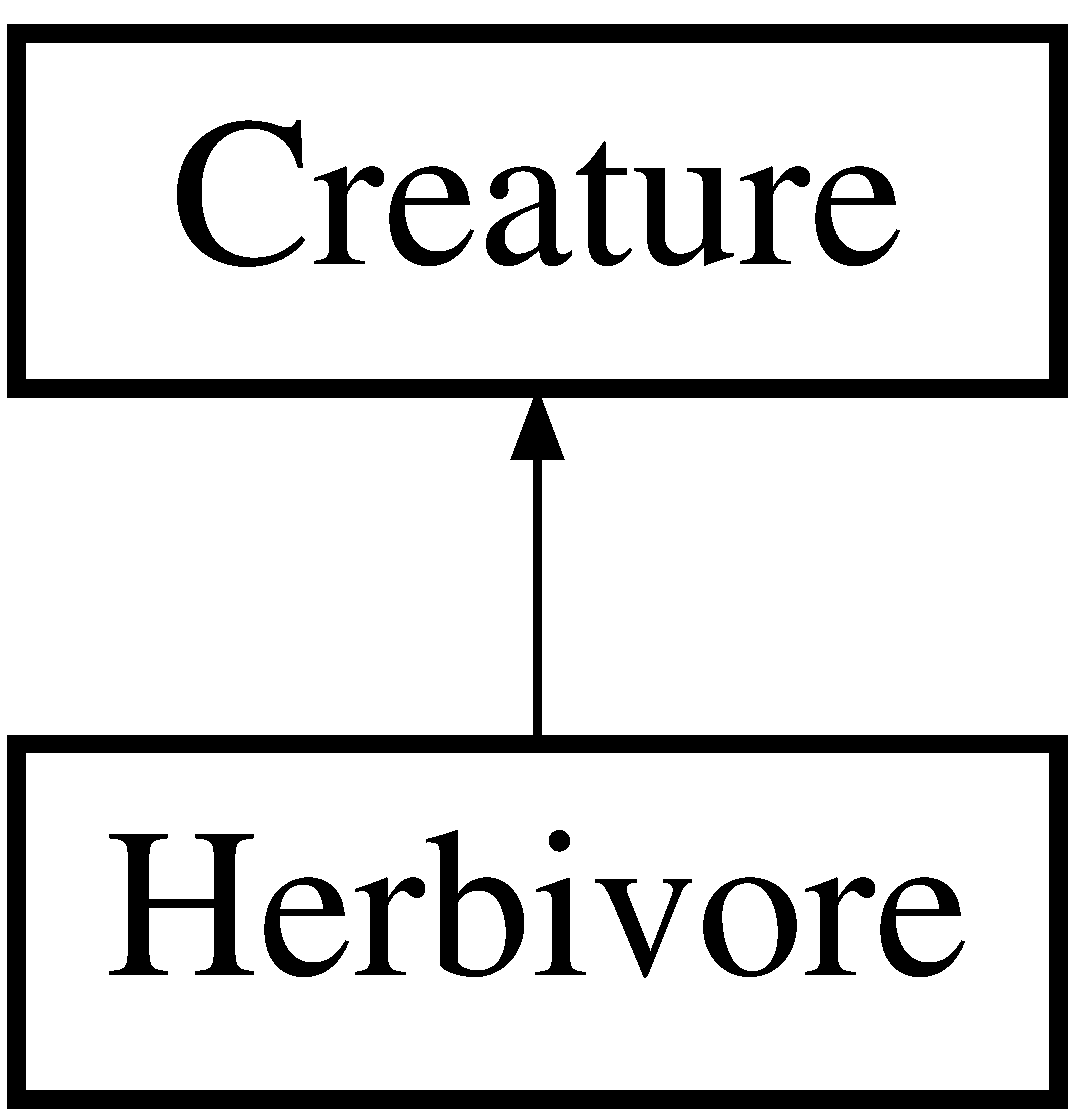
\includegraphics[height=2.000000cm]{class_herbivore}
\end{center}
\end{figure}
\subsection*{Public Member Functions}
\begin{DoxyCompactItemize}
\item 
\mbox{\Hypertarget{class_herbivore_aab17280ff23da5537d7ebffee5d4e4bd}\label{class_herbivore_aab17280ff23da5537d7ebffee5d4e4bd}} 
void {\bfseries herd} ()
\item 
\mbox{\Hypertarget{class_herbivore_a1d428e1f3984436ad6a2985c6f03c451}\label{class_herbivore_a1d428e1f3984436ad6a2985c6f03c451}} 
bool {\bfseries get\+Herding} ()
\end{DoxyCompactItemize}
\subsection*{Additional Inherited Members}


The documentation for this class was generated from the following file\+:\begin{DoxyCompactItemize}
\item 
herbivore.\+h\end{DoxyCompactItemize}

\hypertarget{class_main_window}{}\section{Main\+Window Class Reference}
\label{class_main_window}\index{Main\+Window@{Main\+Window}}
Inheritance diagram for Main\+Window\+:\begin{figure}[H]
\begin{center}
\leavevmode
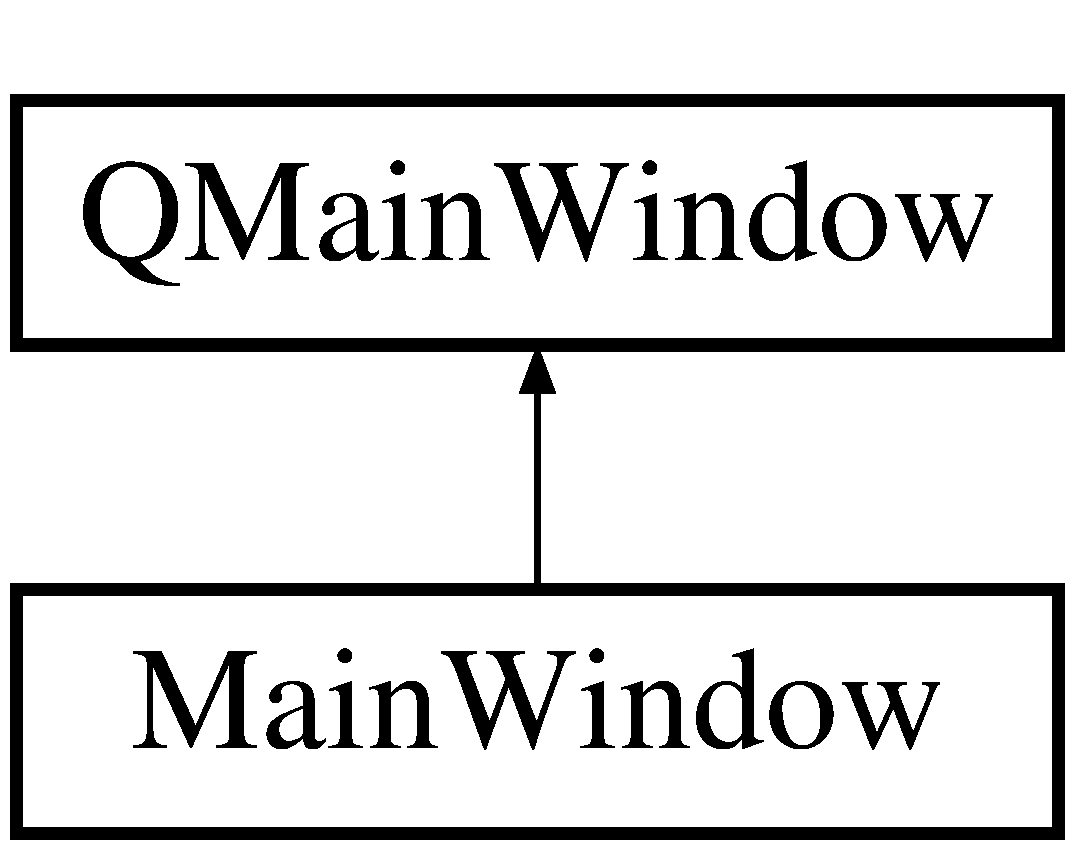
\includegraphics[height=2.000000cm]{class_main_window}
\end{center}
\end{figure}
\subsection*{Classes}
\begin{DoxyCompactItemize}
\item 
struct \hyperlink{struct_main_window_1_1c_coords}{c\+Coords}
\item 
struct \hyperlink{struct_main_window_1_1c_count}{c\+Count}
\end{DoxyCompactItemize}
\subsection*{Public Member Functions}
\begin{DoxyCompactItemize}
\item 
\hyperlink{class_main_window_a8b244be8b7b7db1b08de2a2acb9409db}{Main\+Window} (Q\+Widget $\ast$parent=0)
\item 
\hyperlink{class_main_window_ae98d00a93bc118200eeef9f9bba1dba7}{$\sim$\+Main\+Window} ()
\item 
void \hyperlink{class_main_window_ae6900ae41d5504ba5fd5bebd94c091a8}{count\+Species} (\hyperlink{struct_main_window_1_1c_count}{c\+Count}\mbox{[}$\,$\mbox{]}, \hyperlink{class_creature}{Creature}\mbox{[}$\,$\mbox{]})
\item 
void \hyperlink{class_main_window_a6d41dd2f999fb6fef9b4de0b93e5e93e}{iterate\+Season} (\hyperlink{class_environment}{Environment} \&, \hyperlink{class_creature}{Creature}\mbox{[}$\,$\mbox{]}, \hyperlink{struct_main_window_1_1c_coords}{c\+Coords}\mbox{[}$\,$\mbox{]}, \hyperlink{struct_main_window_1_1c_coords}{c\+Coords}\mbox{[}$\,$\mbox{]}, \hyperlink{struct_main_window_1_1c_coords}{c\+Coords}\mbox{[}$\,$\mbox{]})
\item 
void \hyperlink{class_main_window_a212560b975aacf3247ee109797f99941}{creature\+Instantiation} (\hyperlink{class_environment}{Environment}, \hyperlink{class_creature}{Creature}\mbox{[}$\,$\mbox{]}, \hyperlink{struct_main_window_1_1c_coords}{c\+Coords}\mbox{[}$\,$\mbox{]}, \hyperlink{struct_main_window_1_1c_coords}{c\+Coords}\mbox{[}$\,$\mbox{]}, \hyperlink{struct_main_window_1_1c_coords}{c\+Coords}\mbox{[}$\,$\mbox{]})
\item 
void \hyperlink{class_main_window_a9be9fbd759eb5d1efe76f94d3e16fdc3}{clear\+Dead} (\hyperlink{class_creature}{Creature}\mbox{[}$\,$\mbox{]}, \hyperlink{struct_main_window_1_1c_coords}{c\+Coords}\mbox{[}$\,$\mbox{]}, \hyperlink{struct_main_window_1_1c_coords}{c\+Coords}\mbox{[}$\,$\mbox{]}, \hyperlink{struct_main_window_1_1c_coords}{c\+Coords}\mbox{[}$\,$\mbox{]})
\item 
int \hyperlink{class_main_window_a293a993c9290abb989bedd05501e838d}{translate\+Seed} (string)
\item 
void \hyperlink{class_main_window_abfdebc0fe2713bd3157ea166ab6bb0d5}{run\+Simulation} (int, int)
\end{DoxyCompactItemize}
\subsection*{Public Attributes}
\begin{DoxyCompactItemize}
\item 
\mbox{\Hypertarget{class_main_window_a5a579461e6d3da3db4a95a0c6b42c92b}\label{class_main_window_a5a579461e6d3da3db4a95a0c6b42c92b}} 
bool const {\bfseries P\+R\+I\+N\+T\+\_\+\+C\+R\+E\+A\+T\+U\+R\+ES} = false
\item 
\mbox{\Hypertarget{class_main_window_a286ae12bebf668903a333f39d7223e16}\label{class_main_window_a286ae12bebf668903a333f39d7223e16}} 
bool const {\bfseries P\+R\+I\+N\+T\+\_\+\+D\+E\+B\+U\+G\+\_\+\+H\+U\+NT} = false
\item 
\mbox{\Hypertarget{class_main_window_a0a1ad208278e6125d212f806085ec54e}\label{class_main_window_a0a1ad208278e6125d212f806085ec54e}} 
bool const {\bfseries P\+R\+I\+N\+T\+\_\+\+B\+I\+O\+M\+E\+\_\+\+S\+E\+A\+S\+ON} = true
\item 
\mbox{\Hypertarget{class_main_window_ac044a32e3f8d411066ef2369c47c8244}\label{class_main_window_ac044a32e3f8d411066ef2369c47c8244}} 
bool const {\bfseries D\+E\+B\+U\+G\+\_\+\+P\+L\+OT} = true
\item 
\mbox{\Hypertarget{class_main_window_ab77df82dcce9de9588e733190a6af1f6}\label{class_main_window_ab77df82dcce9de9588e733190a6af1f6}} 
int const {\bfseries N\+U\+M\+S\+P\+E\+C\+I\+ES} = 10
\item 
\mbox{\Hypertarget{class_main_window_a21dee883e6cfca8e664e361c46a10c6b}\label{class_main_window_a21dee883e6cfca8e664e361c46a10c6b}} 
int const {\bfseries N\+U\+M\+C\+R\+E\+A\+T\+U\+R\+ES} = 100
\item 
\mbox{\Hypertarget{class_main_window_a91feb998b7e872bdd0eff4800ab30194}\label{class_main_window_a91feb998b7e872bdd0eff4800ab30194}} 
int {\bfseries N\+U\+M\+S\+E\+A\+S\+O\+NS} = 20
\item 
\mbox{\Hypertarget{class_main_window_ad8ce29de680719ac16dce2f4c8d07ab9}\label{class_main_window_ad8ce29de680719ac16dce2f4c8d07ab9}} 
int const {\bfseries s\+Max} = N\+U\+M\+S\+P\+E\+C\+I\+ES $\ast$ N\+U\+M\+C\+R\+E\+A\+T\+U\+R\+ES $\ast$ 1000
\item 
\mbox{\Hypertarget{class_main_window_ae77061edba8dec4019f3fa23a79a591e}\label{class_main_window_ae77061edba8dec4019f3fa23a79a591e}} 
int {\bfseries s\+Used}
\item 
\mbox{\Hypertarget{class_main_window_ae42dace68680fa2b497199b30a2b198c}\label{class_main_window_ae42dace68680fa2b497199b30a2b198c}} 
int {\bfseries c\+Used}
\item 
\mbox{\Hypertarget{class_main_window_a14056e5221af6e151c12460b6e5e6487}\label{class_main_window_a14056e5221af6e151c12460b6e5e6487}} 
int {\bfseries h\+Used}
\item 
\mbox{\Hypertarget{class_main_window_ae799f62cf4797132d297ec57ba90f7ba}\label{class_main_window_ae799f62cf4797132d297ec57ba90f7ba}} 
int {\bfseries o\+Used}
\item 
\mbox{\Hypertarget{class_main_window_a622e8f757c6c533e46e9cd6c053a0e47}\label{class_main_window_a622e8f757c6c533e46e9cd6c053a0e47}} 
int {\bfseries p\+Used}
\item 
\mbox{\Hypertarget{class_main_window_afb57e3195ba1109e92fd4211eb35d740}\label{class_main_window_afb57e3195ba1109e92fd4211eb35d740}} 
\hyperlink{class_creature}{Creature} $\ast$ {\bfseries s\+List} = N\+U\+LL
\item 
\mbox{\Hypertarget{class_main_window_a0da4e7dbcead644c0ea0a4f643885baf}\label{class_main_window_a0da4e7dbcead644c0ea0a4f643885baf}} 
\hyperlink{struct_main_window_1_1c_coords}{c\+Coords} $\ast$ {\bfseries c\+List} = N\+U\+LL
\item 
\mbox{\Hypertarget{class_main_window_a88ca702f5b1bd1be6343e710f818acc9}\label{class_main_window_a88ca702f5b1bd1be6343e710f818acc9}} 
\hyperlink{struct_main_window_1_1c_coords}{c\+Coords} $\ast$ {\bfseries h\+List} = N\+U\+LL
\item 
\mbox{\Hypertarget{class_main_window_a01a05cc067bb0125eb1ad8e4e883837c}\label{class_main_window_a01a05cc067bb0125eb1ad8e4e883837c}} 
\hyperlink{struct_main_window_1_1c_coords}{c\+Coords} $\ast$ {\bfseries o\+List} = N\+U\+LL
\item 
\mbox{\Hypertarget{class_main_window_a0578b620cc92817cab4480433542e83a}\label{class_main_window_a0578b620cc92817cab4480433542e83a}} 
\hyperlink{struct_main_window_1_1c_count}{c\+Count} $\ast$ {\bfseries plot\+Count} = N\+U\+LL
\item 
\mbox{\Hypertarget{class_main_window_a542517069b2f09f81ca545866509f063}\label{class_main_window_a542517069b2f09f81ca545866509f063}} 
\hyperlink{class_environment}{Environment} {\bfseries Env}
\end{DoxyCompactItemize}


\subsection{Constructor \& Destructor Documentation}
\mbox{\Hypertarget{class_main_window_a8b244be8b7b7db1b08de2a2acb9409db}\label{class_main_window_a8b244be8b7b7db1b08de2a2acb9409db}} 
\index{Main\+Window@{Main\+Window}!Main\+Window@{Main\+Window}}
\index{Main\+Window@{Main\+Window}!Main\+Window@{Main\+Window}}
\subsubsection{\texorpdfstring{Main\+Window()}{MainWindow()}}
{\footnotesize\ttfamily Main\+Window\+::\+Main\+Window (\begin{DoxyParamCaption}\item[{Q\+Widget $\ast$}]{parent = {\ttfamily 0} }\end{DoxyParamCaption})\hspace{0.3cm}{\ttfamily [explicit]}}

Default Constructor. Sets up UI and Detail\+Window for \hyperlink{class_main_window}{Main\+Window}. 
\begin{DoxyParams}{Parameters}
{\em parent} & \\
\hline
\end{DoxyParams}
\begin{DoxyReturn}{Returns}
none 
\end{DoxyReturn}
\mbox{\Hypertarget{class_main_window_ae98d00a93bc118200eeef9f9bba1dba7}\label{class_main_window_ae98d00a93bc118200eeef9f9bba1dba7}} 
\index{Main\+Window@{Main\+Window}!````~Main\+Window@{$\sim$\+Main\+Window}}
\index{````~Main\+Window@{$\sim$\+Main\+Window}!Main\+Window@{Main\+Window}}
\subsubsection{\texorpdfstring{$\sim$\+Main\+Window()}{~MainWindow()}}
{\footnotesize\ttfamily Main\+Window\+::$\sim$\+Main\+Window (\begin{DoxyParamCaption}{ }\end{DoxyParamCaption})}

Destructor for \hyperlink{class_main_window}{Main\+Window}. 
\begin{DoxyParams}{Parameters}
{\em none} & \\
\hline
\end{DoxyParams}
\begin{DoxyReturn}{Returns}
none 
\end{DoxyReturn}


\subsection{Member Function Documentation}
\mbox{\Hypertarget{class_main_window_a9be9fbd759eb5d1efe76f94d3e16fdc3}\label{class_main_window_a9be9fbd759eb5d1efe76f94d3e16fdc3}} 
\index{Main\+Window@{Main\+Window}!clear\+Dead@{clear\+Dead}}
\index{clear\+Dead@{clear\+Dead}!Main\+Window@{Main\+Window}}
\subsubsection{\texorpdfstring{clear\+Dead()}{clearDead()}}
{\footnotesize\ttfamily void Main\+Window\+::clear\+Dead (\begin{DoxyParamCaption}\item[{\hyperlink{class_creature}{Creature}}]{\mbox{[}$\,$\mbox{]},  }\item[{\hyperlink{struct_main_window_1_1c_coords}{c\+Coords}}]{\mbox{[}$\,$\mbox{]},  }\item[{\hyperlink{struct_main_window_1_1c_coords}{c\+Coords}}]{\mbox{[}$\,$\mbox{]},  }\item[{\hyperlink{struct_main_window_1_1c_coords}{c\+Coords}}]{\mbox{[}$\,$\mbox{]} }\end{DoxyParamCaption})}

Method. Clears the numbers of dead creatures. 
\begin{DoxyParams}{Parameters}
{\em s\+List} & \\
\hline
{\em c\+List} & \\
\hline
{\em o\+List} & \\
\hline
{\em h\+List} & \\
\hline
\end{DoxyParams}
\begin{DoxyReturn}{Returns}
none 
\end{DoxyReturn}
\mbox{\Hypertarget{class_main_window_ae6900ae41d5504ba5fd5bebd94c091a8}\label{class_main_window_ae6900ae41d5504ba5fd5bebd94c091a8}} 
\index{Main\+Window@{Main\+Window}!count\+Species@{count\+Species}}
\index{count\+Species@{count\+Species}!Main\+Window@{Main\+Window}}
\subsubsection{\texorpdfstring{count\+Species()}{countSpecies()}}
{\footnotesize\ttfamily void Main\+Window\+::count\+Species (\begin{DoxyParamCaption}\item[{\hyperlink{struct_main_window_1_1c_count}{c\+Count}}]{\mbox{[}$\,$\mbox{]},  }\item[{\hyperlink{class_creature}{Creature}}]{\mbox{[}$\,$\mbox{]} }\end{DoxyParamCaption})}

Method. Gets the total counts for a species. 
\begin{DoxyParams}{Parameters}
{\em c\+Count\mbox{[}$\,$\mbox{]}} & \\
\hline
{\em Creature\mbox{[}$\,$\mbox{]}} & \\
\hline
\end{DoxyParams}
\begin{DoxyReturn}{Returns}
none 
\end{DoxyReturn}
\mbox{\Hypertarget{class_main_window_a212560b975aacf3247ee109797f99941}\label{class_main_window_a212560b975aacf3247ee109797f99941}} 
\index{Main\+Window@{Main\+Window}!creature\+Instantiation@{creature\+Instantiation}}
\index{creature\+Instantiation@{creature\+Instantiation}!Main\+Window@{Main\+Window}}
\subsubsection{\texorpdfstring{creature\+Instantiation()}{creatureInstantiation()}}
{\footnotesize\ttfamily void Main\+Window\+::creature\+Instantiation (\begin{DoxyParamCaption}\item[{\hyperlink{class_environment}{Environment}}]{Env,  }\item[{\hyperlink{class_creature}{Creature}}]{s\+List\mbox{[}$\,$\mbox{]},  }\item[{\hyperlink{struct_main_window_1_1c_coords}{c\+Coords}}]{c\+List\mbox{[}$\,$\mbox{]},  }\item[{\hyperlink{struct_main_window_1_1c_coords}{c\+Coords}}]{h\+List\mbox{[}$\,$\mbox{]},  }\item[{\hyperlink{struct_main_window_1_1c_coords}{c\+Coords}}]{o\+List\mbox{[}$\,$\mbox{]} }\end{DoxyParamCaption})}

Method. Instantiates creatures for a simulation. 
\begin{DoxyParams}{Parameters}
{\em Env} & \\
\hline
{\em s\+List} & \\
\hline
{\em c\+List} & \\
\hline
{\em h\+List} & \\
\hline
{\em o\+List} & \\
\hline
\end{DoxyParams}
\begin{DoxyReturn}{Returns}
none 
\end{DoxyReturn}
\mbox{\Hypertarget{class_main_window_a6d41dd2f999fb6fef9b4de0b93e5e93e}\label{class_main_window_a6d41dd2f999fb6fef9b4de0b93e5e93e}} 
\index{Main\+Window@{Main\+Window}!iterate\+Season@{iterate\+Season}}
\index{iterate\+Season@{iterate\+Season}!Main\+Window@{Main\+Window}}
\subsubsection{\texorpdfstring{iterate\+Season()}{iterateSeason()}}
{\footnotesize\ttfamily void Main\+Window\+::iterate\+Season (\begin{DoxyParamCaption}\item[{\hyperlink{class_environment}{Environment} \&}]{Env,  }\item[{\hyperlink{class_creature}{Creature}}]{s\+List\mbox{[}$\,$\mbox{]},  }\item[{\hyperlink{struct_main_window_1_1c_coords}{c\+Coords}}]{c\+List\mbox{[}$\,$\mbox{]},  }\item[{\hyperlink{struct_main_window_1_1c_coords}{c\+Coords}}]{o\+List\mbox{[}$\,$\mbox{]},  }\item[{\hyperlink{struct_main_window_1_1c_coords}{c\+Coords}}]{h\+List\mbox{[}$\,$\mbox{]} }\end{DoxyParamCaption})}

Method. Iterates the season for the simulation. 
\begin{DoxyParams}{Parameters}
{\em Env} & \\
\hline
{\em s\+List} & \\
\hline
{\em c\+List} & \\
\hline
{\em o\+List} & \\
\hline
{\em h\+List} & \\
\hline
\end{DoxyParams}
\begin{DoxyReturn}{Returns}
none 
\end{DoxyReturn}
\mbox{\Hypertarget{class_main_window_abfdebc0fe2713bd3157ea166ab6bb0d5}\label{class_main_window_abfdebc0fe2713bd3157ea166ab6bb0d5}} 
\index{Main\+Window@{Main\+Window}!run\+Simulation@{run\+Simulation}}
\index{run\+Simulation@{run\+Simulation}!Main\+Window@{Main\+Window}}
\subsubsection{\texorpdfstring{run\+Simulation()}{runSimulation()}}
{\footnotesize\ttfamily void Main\+Window\+::run\+Simulation (\begin{DoxyParamCaption}\item[{int}]{num\+Iterations,  }\item[{int}]{seed }\end{DoxyParamCaption})}

Method. Runs the simulation for the program. 
\begin{DoxyParams}{Parameters}
{\em num\+Iterations} & \\
\hline
{\em seed} & \\
\hline
\end{DoxyParams}
\begin{DoxyReturn}{Returns}
none 
\end{DoxyReturn}
\mbox{\Hypertarget{class_main_window_a293a993c9290abb989bedd05501e838d}\label{class_main_window_a293a993c9290abb989bedd05501e838d}} 
\index{Main\+Window@{Main\+Window}!translate\+Seed@{translate\+Seed}}
\index{translate\+Seed@{translate\+Seed}!Main\+Window@{Main\+Window}}
\subsubsection{\texorpdfstring{translate\+Seed()}{translateSeed()}}
{\footnotesize\ttfamily int Main\+Window\+::translate\+Seed (\begin{DoxyParamCaption}\item[{string}]{user\+Seed }\end{DoxyParamCaption})}

Method. Translates seed into an integer value. 
\begin{DoxyParams}{Parameters}
{\em user\+Seed} & \\
\hline
\end{DoxyParams}
\begin{DoxyReturn}{Returns}
seed 
\end{DoxyReturn}


The documentation for this class was generated from the following files\+:\begin{DoxyCompactItemize}
\item 
mainwindow.\+h\item 
mainwindow.\+cpp\end{DoxyCompactItemize}

\hypertarget{class_omnivore}{}\section{Omnivore Class Reference}
\label{class_omnivore}\index{Omnivore@{Omnivore}}
Inheritance diagram for Omnivore\+:\begin{figure}[H]
\begin{center}
\leavevmode
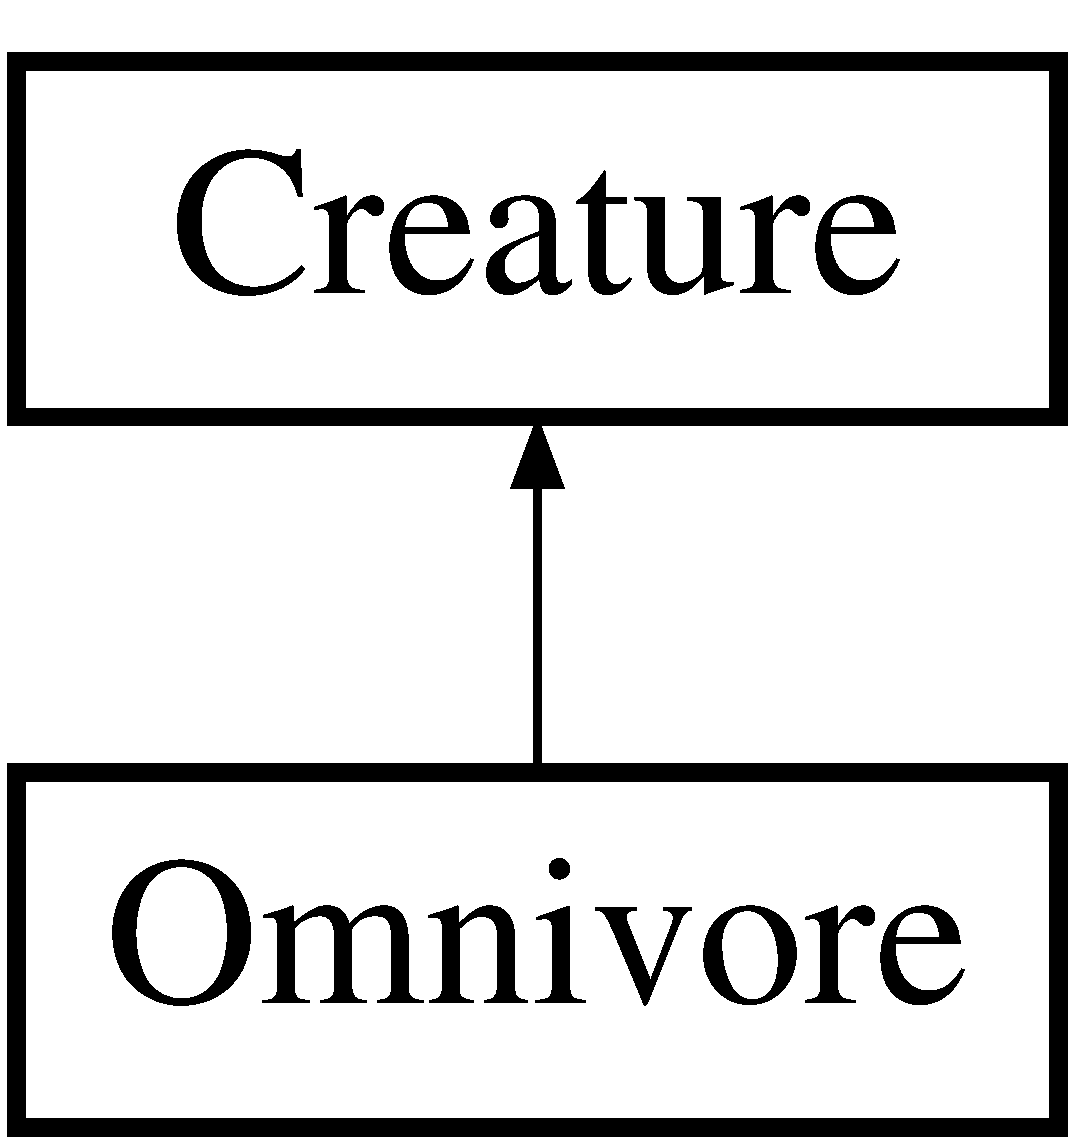
\includegraphics[height=2.000000cm]{class_omnivore}
\end{center}
\end{figure}
\subsection*{Public Member Functions}
\begin{DoxyCompactItemize}
\item 
\mbox{\Hypertarget{class_omnivore_ad8ddc3f954b778f6a628c19c0fa6d6c9}\label{class_omnivore_ad8ddc3f954b778f6a628c19c0fa6d6c9}} 
{\bfseries Omnivore} (\hyperlink{class_creature}{Creature} \&creature)
\item 
\mbox{\Hypertarget{class_omnivore_a24b519d8b584fa889241e0eb8d666b2e}\label{class_omnivore_a24b519d8b584fa889241e0eb8d666b2e}} 
bool {\bfseries hunt} (\hyperlink{class_creature}{Creature} \&prey)
\item 
\mbox{\Hypertarget{class_omnivore_a9e962a0697c4d09297c8edffce538b3e}\label{class_omnivore_a9e962a0697c4d09297c8edffce538b3e}} 
bool {\bfseries hunt} (\hyperlink{class_herbivore}{Herbivore} prey)
\item 
\mbox{\Hypertarget{class_omnivore_a27a01e0439cff6ace454a11a0e9a4fe0}\label{class_omnivore_a27a01e0439cff6ace454a11a0e9a4fe0}} 
bool {\bfseries hunt} (\hyperlink{class_omnivore}{Omnivore} prey)
\item 
\mbox{\Hypertarget{class_omnivore_ab6a1b337eb581e9484435cfabbbb2b57}\label{class_omnivore_ab6a1b337eb581e9484435cfabbbb2b57}} 
void {\bfseries herd} ()
\item 
\mbox{\Hypertarget{class_omnivore_a32a33697de9a2e666a38a3ce69f6f803}\label{class_omnivore_a32a33697de9a2e666a38a3ce69f6f803}} 
bool {\bfseries get\+Herding} ()
\end{DoxyCompactItemize}
\subsection*{Additional Inherited Members}


The documentation for this class was generated from the following file\+:\begin{DoxyCompactItemize}
\item 
omnivore.\+h\end{DoxyCompactItemize}

\hypertarget{structseasons}{}\section{seasons Struct Reference}
\label{structseasons}\index{seasons@{seasons}}
\subsection*{Public Attributes}
\begin{DoxyCompactItemize}
\item 
\mbox{\Hypertarget{structseasons_a64ee7f79620419786e3968f686111823}\label{structseasons_a64ee7f79620419786e3968f686111823}} 
float {\bfseries water\+\_\+supply\+\_\+m}
\item 
\mbox{\Hypertarget{structseasons_aed69f632e642ef16f4c620efc8a1922f}\label{structseasons_aed69f632e642ef16f4c620efc8a1922f}} 
float {\bfseries water\+\_\+refill\+\_\+m}
\end{DoxyCompactItemize}


The documentation for this struct was generated from the following file\+:\begin{DoxyCompactItemize}
\item 
environment.\+h\end{DoxyCompactItemize}

\hypertarget{class_trait}{}\section{Trait Class Reference}
\label{class_trait}\index{Trait@{Trait}}
\subsection*{Public Member Functions}
\begin{DoxyCompactItemize}
\item 
\hyperlink{class_trait_aae36b201023c346213c0e5bcc1c7922f}{Trait} ()
\item 
\mbox{\Hypertarget{class_trait_a58e7f2810d1eeae90a86ef44c8226642}\label{class_trait_a58e7f2810d1eeae90a86ef44c8226642}} 
{\bfseries Trait} (string, float, float, float, float, float, float)
\item 
virtual \hyperlink{class_trait_a28ec215ff3fac94d1657088fee6007a4}{$\sim$\+Trait} ()
\item 
float \hyperlink{class_trait_a7bd7db0c5b950d44aff9ca4943eef187}{get\+Temp\+Resist} ()
\item 
float \hyperlink{class_trait_a4d065437505563d16c1f5cae912d8383}{get\+Disease\+Resist} ()
\item 
float \hyperlink{class_trait_a4275bb208c1fdcb232251d7014b7a9dc}{get\+Predator\+Resist} ()
\item 
float \hyperlink{class_trait_a28ded6c3488a3e8704173bf039bfa936}{get\+Breed\+Chance} ()
\item 
float \hyperlink{class_trait_abc05dc8d331b54d5d9d080a2507efa39}{get\+Herd\+Tendency} ()
\item 
float \hyperlink{class_trait_a169f7d0c6ccb29e5d385c33cc8a87e52}{get\+Water\+Need} ()
\item 
string \hyperlink{class_trait_a4e4fa9d379a0e7f36f1d1577ebd487a0}{get\+Trait\+Name} ()
\item 
bool \hyperlink{class_trait_af5cd74fadebbb43800c2ae93a5007de1}{get\+Dominance} ()
\item 
int \hyperlink{class_trait_ac1bcf9cebceb67efe5c60cf04f85a383}{get\+Animal\+Type} ()
\item 
int \hyperlink{class_trait_a285974c25162993ff108a762b1e5472c}{get\+Type} ()
\item 
void \hyperlink{class_trait_ac0a31db1a9d59ffbbdcb55d58aefbaea}{set\+Trait\+Name} (string)
\item 
void \hyperlink{class_trait_aa8b92de8273b52045e4a545e2bbd4075}{set\+Dominance} (bool)
\item 
void \hyperlink{class_trait_a4502b8d4b670a9aa39a49cfa394e31e1}{set\+Animal\+Type} (int)
\item 
void \hyperlink{class_trait_afb95de8d08b9e6509d670af19db03d9d}{set\+Temp\+Resist} (float)
\item 
void \hyperlink{class_trait_afd78c8d97e46ea8ba6b8240034419b1b}{set\+Disease\+Resist} (float)
\item 
void \hyperlink{class_trait_a952e008b31b2da8206319fd8b5bc4409}{set\+Predator\+Resist} (float)
\item 
void \hyperlink{class_trait_aec781297ddedcbec15a369453fea9557}{set\+Breed\+Chance} (float)
\item 
void \hyperlink{class_trait_ab5881ed05c689ee84de9997aa7243478}{set\+Herd\+Tendency} (float)
\item 
void \hyperlink{class_trait_abba488e319c1419698d6d991c70f5900}{set\+Water\+Need} (float)
\item 
void \hyperlink{class_trait_a4409499a3a87f38106272489ecab2007}{set\+Type} (int)
\item 
string \hyperlink{class_trait_a035698aed4673b26e21e9d8d787fe3dc}{to\+String} ()
\item 
bool \hyperlink{class_trait_abe35dcc6c7da6345d3f862082cc7f956}{operator$>$=} (const \hyperlink{class_trait}{Trait} \&) const
\item 
bool \hyperlink{class_trait_a04b0daee14f5cfd70e7e5ac485ce87ec}{operator==} (const \hyperlink{class_trait}{Trait} \&) const
\item 
void \hyperlink{class_trait_a88a21860c203813df4ecdcfe37758f88}{operator=} (const \hyperlink{class_trait}{Trait} \&)
\end{DoxyCompactItemize}


\subsection{Constructor \& Destructor Documentation}
\mbox{\Hypertarget{class_trait_aae36b201023c346213c0e5bcc1c7922f}\label{class_trait_aae36b201023c346213c0e5bcc1c7922f}} 
\index{Trait@{Trait}!Trait@{Trait}}
\index{Trait@{Trait}!Trait@{Trait}}
\subsubsection{\texorpdfstring{Trait()}{Trait()}}
{\footnotesize\ttfamily Trait\+::\+Trait (\begin{DoxyParamCaption}{ }\end{DoxyParamCaption})}

Default Constructor. 
\begin{DoxyParams}{Parameters}
{\em none} & \\
\hline
\end{DoxyParams}
\mbox{\Hypertarget{class_trait_a28ec215ff3fac94d1657088fee6007a4}\label{class_trait_a28ec215ff3fac94d1657088fee6007a4}} 
\index{Trait@{Trait}!````~Trait@{$\sim$\+Trait}}
\index{````~Trait@{$\sim$\+Trait}!Trait@{Trait}}
\subsubsection{\texorpdfstring{$\sim$\+Trait()}{~Trait()}}
{\footnotesize\ttfamily Trait\+::$\sim$\+Trait (\begin{DoxyParamCaption}{ }\end{DoxyParamCaption})\hspace{0.3cm}{\ttfamily [virtual]}}

Destructor. 
\begin{DoxyParams}{Parameters}
{\em none} & \\
\hline
\end{DoxyParams}


\subsection{Member Function Documentation}
\mbox{\Hypertarget{class_trait_ac1bcf9cebceb67efe5c60cf04f85a383}\label{class_trait_ac1bcf9cebceb67efe5c60cf04f85a383}} 
\index{Trait@{Trait}!get\+Animal\+Type@{get\+Animal\+Type}}
\index{get\+Animal\+Type@{get\+Animal\+Type}!Trait@{Trait}}
\subsubsection{\texorpdfstring{get\+Animal\+Type()}{getAnimalType()}}
{\footnotesize\ttfamily int Trait\+::get\+Animal\+Type (\begin{DoxyParamCaption}{ }\end{DoxyParamCaption})}

Getter. Returns type of creature. 
\begin{DoxyParams}{Parameters}
{\em none} & \\
\hline
\end{DoxyParams}
\begin{DoxyReturn}{Returns}
animal\+Type 
\end{DoxyReturn}
\mbox{\Hypertarget{class_trait_a28ded6c3488a3e8704173bf039bfa936}\label{class_trait_a28ded6c3488a3e8704173bf039bfa936}} 
\index{Trait@{Trait}!get\+Breed\+Chance@{get\+Breed\+Chance}}
\index{get\+Breed\+Chance@{get\+Breed\+Chance}!Trait@{Trait}}
\subsubsection{\texorpdfstring{get\+Breed\+Chance()}{getBreedChance()}}
{\footnotesize\ttfamily float Trait\+::get\+Breed\+Chance (\begin{DoxyParamCaption}{ }\end{DoxyParamCaption})}

Getter. Returns breed chance. 
\begin{DoxyParams}{Parameters}
{\em none} & \\
\hline
\end{DoxyParams}
\begin{DoxyReturn}{Returns}
breed\+Chance 
\end{DoxyReturn}
\mbox{\Hypertarget{class_trait_a4d065437505563d16c1f5cae912d8383}\label{class_trait_a4d065437505563d16c1f5cae912d8383}} 
\index{Trait@{Trait}!get\+Disease\+Resist@{get\+Disease\+Resist}}
\index{get\+Disease\+Resist@{get\+Disease\+Resist}!Trait@{Trait}}
\subsubsection{\texorpdfstring{get\+Disease\+Resist()}{getDiseaseResist()}}
{\footnotesize\ttfamily float Trait\+::get\+Disease\+Resist (\begin{DoxyParamCaption}{ }\end{DoxyParamCaption})}

Getter. Returns disease resistance. 
\begin{DoxyParams}{Parameters}
{\em none} & \\
\hline
\end{DoxyParams}
\begin{DoxyReturn}{Returns}
disease\+\_\+resist 
\end{DoxyReturn}
\mbox{\Hypertarget{class_trait_af5cd74fadebbb43800c2ae93a5007de1}\label{class_trait_af5cd74fadebbb43800c2ae93a5007de1}} 
\index{Trait@{Trait}!get\+Dominance@{get\+Dominance}}
\index{get\+Dominance@{get\+Dominance}!Trait@{Trait}}
\subsubsection{\texorpdfstring{get\+Dominance()}{getDominance()}}
{\footnotesize\ttfamily bool Trait\+::get\+Dominance (\begin{DoxyParamCaption}{ }\end{DoxyParamCaption})}

Getter. Returns dominance of trait. 
\begin{DoxyParams}{Parameters}
{\em none} & \\
\hline
\end{DoxyParams}
\begin{DoxyReturn}{Returns}
dominance 
\end{DoxyReturn}
\mbox{\Hypertarget{class_trait_abc05dc8d331b54d5d9d080a2507efa39}\label{class_trait_abc05dc8d331b54d5d9d080a2507efa39}} 
\index{Trait@{Trait}!get\+Herd\+Tendency@{get\+Herd\+Tendency}}
\index{get\+Herd\+Tendency@{get\+Herd\+Tendency}!Trait@{Trait}}
\subsubsection{\texorpdfstring{get\+Herd\+Tendency()}{getHerdTendency()}}
{\footnotesize\ttfamily float Trait\+::get\+Herd\+Tendency (\begin{DoxyParamCaption}{ }\end{DoxyParamCaption})}

Getter. Returns herd tendency. 
\begin{DoxyParams}{Parameters}
{\em none} & \\
\hline
\end{DoxyParams}
\begin{DoxyReturn}{Returns}
herd\+Tendency 
\end{DoxyReturn}
\mbox{\Hypertarget{class_trait_a4275bb208c1fdcb232251d7014b7a9dc}\label{class_trait_a4275bb208c1fdcb232251d7014b7a9dc}} 
\index{Trait@{Trait}!get\+Predator\+Resist@{get\+Predator\+Resist}}
\index{get\+Predator\+Resist@{get\+Predator\+Resist}!Trait@{Trait}}
\subsubsection{\texorpdfstring{get\+Predator\+Resist()}{getPredatorResist()}}
{\footnotesize\ttfamily float Trait\+::get\+Predator\+Resist (\begin{DoxyParamCaption}{ }\end{DoxyParamCaption})}

Getter. Returns predator resistance. 
\begin{DoxyParams}{Parameters}
{\em none} & \\
\hline
\end{DoxyParams}
\begin{DoxyReturn}{Returns}
predator\+\_\+resist 
\end{DoxyReturn}
\mbox{\Hypertarget{class_trait_a7bd7db0c5b950d44aff9ca4943eef187}\label{class_trait_a7bd7db0c5b950d44aff9ca4943eef187}} 
\index{Trait@{Trait}!get\+Temp\+Resist@{get\+Temp\+Resist}}
\index{get\+Temp\+Resist@{get\+Temp\+Resist}!Trait@{Trait}}
\subsubsection{\texorpdfstring{get\+Temp\+Resist()}{getTempResist()}}
{\footnotesize\ttfamily float Trait\+::get\+Temp\+Resist (\begin{DoxyParamCaption}{ }\end{DoxyParamCaption})}

Getter. Returns temperature resistance. 
\begin{DoxyParams}{Parameters}
{\em none} & \\
\hline
\end{DoxyParams}
\begin{DoxyReturn}{Returns}
temp\+\_\+resist 
\end{DoxyReturn}
\mbox{\Hypertarget{class_trait_a4e4fa9d379a0e7f36f1d1577ebd487a0}\label{class_trait_a4e4fa9d379a0e7f36f1d1577ebd487a0}} 
\index{Trait@{Trait}!get\+Trait\+Name@{get\+Trait\+Name}}
\index{get\+Trait\+Name@{get\+Trait\+Name}!Trait@{Trait}}
\subsubsection{\texorpdfstring{get\+Trait\+Name()}{getTraitName()}}
{\footnotesize\ttfamily string Trait\+::get\+Trait\+Name (\begin{DoxyParamCaption}{ }\end{DoxyParamCaption})}

Getter. Returns name for trait. 
\begin{DoxyParams}{Parameters}
{\em none} & \\
\hline
\end{DoxyParams}
\begin{DoxyReturn}{Returns}
trait\+\_\+name 
\end{DoxyReturn}
\mbox{\Hypertarget{class_trait_a285974c25162993ff108a762b1e5472c}\label{class_trait_a285974c25162993ff108a762b1e5472c}} 
\index{Trait@{Trait}!get\+Type@{get\+Type}}
\index{get\+Type@{get\+Type}!Trait@{Trait}}
\subsubsection{\texorpdfstring{get\+Type()}{getType()}}
{\footnotesize\ttfamily int Trait\+::get\+Type (\begin{DoxyParamCaption}{ }\end{DoxyParamCaption})}

Getter. Returns type of trait. 
\begin{DoxyParams}{Parameters}
{\em none} & \\
\hline
\end{DoxyParams}
\begin{DoxyReturn}{Returns}
type 
\end{DoxyReturn}
\mbox{\Hypertarget{class_trait_a169f7d0c6ccb29e5d385c33cc8a87e52}\label{class_trait_a169f7d0c6ccb29e5d385c33cc8a87e52}} 
\index{Trait@{Trait}!get\+Water\+Need@{get\+Water\+Need}}
\index{get\+Water\+Need@{get\+Water\+Need}!Trait@{Trait}}
\subsubsection{\texorpdfstring{get\+Water\+Need()}{getWaterNeed()}}
{\footnotesize\ttfamily float Trait\+::get\+Water\+Need (\begin{DoxyParamCaption}{ }\end{DoxyParamCaption})}

Getter. Returns need for water. 
\begin{DoxyParams}{Parameters}
{\em none} & \\
\hline
\end{DoxyParams}
\begin{DoxyReturn}{Returns}
water\+Need 
\end{DoxyReturn}
\mbox{\Hypertarget{class_trait_a88a21860c203813df4ecdcfe37758f88}\label{class_trait_a88a21860c203813df4ecdcfe37758f88}} 
\index{Trait@{Trait}!operator=@{operator=}}
\index{operator=@{operator=}!Trait@{Trait}}
\subsubsection{\texorpdfstring{operator=()}{operator=()}}
{\footnotesize\ttfamily void Trait\+::operator= (\begin{DoxyParamCaption}\item[{const \hyperlink{class_trait}{Trait} \&}]{other }\end{DoxyParamCaption})}

Method. Sets a trait to another. 
\begin{DoxyParams}{Parameters}
{\em other} & \\
\hline
\end{DoxyParams}
\begin{DoxyReturn}{Returns}
none 
\end{DoxyReturn}
\mbox{\Hypertarget{class_trait_a04b0daee14f5cfd70e7e5ac485ce87ec}\label{class_trait_a04b0daee14f5cfd70e7e5ac485ce87ec}} 
\index{Trait@{Trait}!operator==@{operator==}}
\index{operator==@{operator==}!Trait@{Trait}}
\subsubsection{\texorpdfstring{operator==()}{operator==()}}
{\footnotesize\ttfamily bool Trait\+::operator== (\begin{DoxyParamCaption}\item[{const \hyperlink{class_trait}{Trait} \&}]{other }\end{DoxyParamCaption}) const}

Method. Checks to see if two traits are equivalent. 
\begin{DoxyParams}{Parameters}
{\em other} & \\
\hline
\end{DoxyParams}
\begin{DoxyReturn}{Returns}
boolean 
\end{DoxyReturn}
\mbox{\Hypertarget{class_trait_abe35dcc6c7da6345d3f862082cc7f956}\label{class_trait_abe35dcc6c7da6345d3f862082cc7f956}} 
\index{Trait@{Trait}!operator$>$=@{operator$>$=}}
\index{operator$>$=@{operator$>$=}!Trait@{Trait}}
\subsubsection{\texorpdfstring{operator$>$=()}{operator>=()}}
{\footnotesize\ttfamily bool Trait\+::operator$>$= (\begin{DoxyParamCaption}\item[{const \hyperlink{class_trait}{Trait} \&}]{other }\end{DoxyParamCaption}) const}

Method. Checks if a trait is greater than or equivalent to another. 
\begin{DoxyParams}{Parameters}
{\em other} & \\
\hline
\end{DoxyParams}
\begin{DoxyReturn}{Returns}
boolean 
\end{DoxyReturn}
\mbox{\Hypertarget{class_trait_a4502b8d4b670a9aa39a49cfa394e31e1}\label{class_trait_a4502b8d4b670a9aa39a49cfa394e31e1}} 
\index{Trait@{Trait}!set\+Animal\+Type@{set\+Animal\+Type}}
\index{set\+Animal\+Type@{set\+Animal\+Type}!Trait@{Trait}}
\subsubsection{\texorpdfstring{set\+Animal\+Type()}{setAnimalType()}}
{\footnotesize\ttfamily void Trait\+::set\+Animal\+Type (\begin{DoxyParamCaption}\item[{int}]{type }\end{DoxyParamCaption})}

Setter. Sets the type of animal. 
\begin{DoxyParams}{Parameters}
{\em type} & \\
\hline
\end{DoxyParams}
\begin{DoxyReturn}{Returns}
none 
\end{DoxyReturn}
\mbox{\Hypertarget{class_trait_aec781297ddedcbec15a369453fea9557}\label{class_trait_aec781297ddedcbec15a369453fea9557}} 
\index{Trait@{Trait}!set\+Breed\+Chance@{set\+Breed\+Chance}}
\index{set\+Breed\+Chance@{set\+Breed\+Chance}!Trait@{Trait}}
\subsubsection{\texorpdfstring{set\+Breed\+Chance()}{setBreedChance()}}
{\footnotesize\ttfamily void Trait\+::set\+Breed\+Chance (\begin{DoxyParamCaption}\item[{float}]{bc }\end{DoxyParamCaption})}

Setter. Sets breed chance based on trait. 
\begin{DoxyParams}{Parameters}
{\em bc} & \\
\hline
\end{DoxyParams}
\begin{DoxyReturn}{Returns}
none 
\end{DoxyReturn}
\mbox{\Hypertarget{class_trait_afd78c8d97e46ea8ba6b8240034419b1b}\label{class_trait_afd78c8d97e46ea8ba6b8240034419b1b}} 
\index{Trait@{Trait}!set\+Disease\+Resist@{set\+Disease\+Resist}}
\index{set\+Disease\+Resist@{set\+Disease\+Resist}!Trait@{Trait}}
\subsubsection{\texorpdfstring{set\+Disease\+Resist()}{setDiseaseResist()}}
{\footnotesize\ttfamily void Trait\+::set\+Disease\+Resist (\begin{DoxyParamCaption}\item[{float}]{dr }\end{DoxyParamCaption})}

Setter. Sets disease resistance based on trait. 
\begin{DoxyParams}{Parameters}
{\em dr} & \\
\hline
\end{DoxyParams}
\begin{DoxyReturn}{Returns}
none 
\end{DoxyReturn}
\mbox{\Hypertarget{class_trait_aa8b92de8273b52045e4a545e2bbd4075}\label{class_trait_aa8b92de8273b52045e4a545e2bbd4075}} 
\index{Trait@{Trait}!set\+Dominance@{set\+Dominance}}
\index{set\+Dominance@{set\+Dominance}!Trait@{Trait}}
\subsubsection{\texorpdfstring{set\+Dominance()}{setDominance()}}
{\footnotesize\ttfamily void Trait\+::set\+Dominance (\begin{DoxyParamCaption}\item[{bool}]{dom }\end{DoxyParamCaption})}

Setter. Sets dominance of a trait. 
\begin{DoxyParams}{Parameters}
{\em dom} & \\
\hline
\end{DoxyParams}
\begin{DoxyReturn}{Returns}
none 
\end{DoxyReturn}
\mbox{\Hypertarget{class_trait_ab5881ed05c689ee84de9997aa7243478}\label{class_trait_ab5881ed05c689ee84de9997aa7243478}} 
\index{Trait@{Trait}!set\+Herd\+Tendency@{set\+Herd\+Tendency}}
\index{set\+Herd\+Tendency@{set\+Herd\+Tendency}!Trait@{Trait}}
\subsubsection{\texorpdfstring{set\+Herd\+Tendency()}{setHerdTendency()}}
{\footnotesize\ttfamily void Trait\+::set\+Herd\+Tendency (\begin{DoxyParamCaption}\item[{float}]{ht }\end{DoxyParamCaption})}

Setter. Sets herd tendency based on trait. 
\begin{DoxyParams}{Parameters}
{\em ht} & \\
\hline
\end{DoxyParams}
\begin{DoxyReturn}{Returns}
none 
\end{DoxyReturn}
\mbox{\Hypertarget{class_trait_a952e008b31b2da8206319fd8b5bc4409}\label{class_trait_a952e008b31b2da8206319fd8b5bc4409}} 
\index{Trait@{Trait}!set\+Predator\+Resist@{set\+Predator\+Resist}}
\index{set\+Predator\+Resist@{set\+Predator\+Resist}!Trait@{Trait}}
\subsubsection{\texorpdfstring{set\+Predator\+Resist()}{setPredatorResist()}}
{\footnotesize\ttfamily void Trait\+::set\+Predator\+Resist (\begin{DoxyParamCaption}\item[{float}]{pr }\end{DoxyParamCaption})}

Setter. Sets predator resistance based on trait. 
\begin{DoxyParams}{Parameters}
{\em pr} & \\
\hline
\end{DoxyParams}
\begin{DoxyReturn}{Returns}
none 
\end{DoxyReturn}
\mbox{\Hypertarget{class_trait_afb95de8d08b9e6509d670af19db03d9d}\label{class_trait_afb95de8d08b9e6509d670af19db03d9d}} 
\index{Trait@{Trait}!set\+Temp\+Resist@{set\+Temp\+Resist}}
\index{set\+Temp\+Resist@{set\+Temp\+Resist}!Trait@{Trait}}
\subsubsection{\texorpdfstring{set\+Temp\+Resist()}{setTempResist()}}
{\footnotesize\ttfamily void Trait\+::set\+Temp\+Resist (\begin{DoxyParamCaption}\item[{float}]{tr }\end{DoxyParamCaption})}

Setter. Sets temperature resistance based on trait. 
\begin{DoxyParams}{Parameters}
{\em tr} & \\
\hline
\end{DoxyParams}
\begin{DoxyReturn}{Returns}
none 
\end{DoxyReturn}
\mbox{\Hypertarget{class_trait_ac0a31db1a9d59ffbbdcb55d58aefbaea}\label{class_trait_ac0a31db1a9d59ffbbdcb55d58aefbaea}} 
\index{Trait@{Trait}!set\+Trait\+Name@{set\+Trait\+Name}}
\index{set\+Trait\+Name@{set\+Trait\+Name}!Trait@{Trait}}
\subsubsection{\texorpdfstring{set\+Trait\+Name()}{setTraitName()}}
{\footnotesize\ttfamily void Trait\+::set\+Trait\+Name (\begin{DoxyParamCaption}\item[{string}]{name }\end{DoxyParamCaption})}

Setter. Sets trait name. 
\begin{DoxyParams}{Parameters}
{\em name} & \\
\hline
\end{DoxyParams}
\begin{DoxyReturn}{Returns}
none 
\end{DoxyReturn}
\mbox{\Hypertarget{class_trait_a4409499a3a87f38106272489ecab2007}\label{class_trait_a4409499a3a87f38106272489ecab2007}} 
\index{Trait@{Trait}!set\+Type@{set\+Type}}
\index{set\+Type@{set\+Type}!Trait@{Trait}}
\subsubsection{\texorpdfstring{set\+Type()}{setType()}}
{\footnotesize\ttfamily void Trait\+::set\+Type (\begin{DoxyParamCaption}\item[{int}]{i }\end{DoxyParamCaption})}

Setter. Sets type. 
\begin{DoxyParams}{Parameters}
{\em i} & \\
\hline
\end{DoxyParams}
\begin{DoxyReturn}{Returns}
none 
\end{DoxyReturn}
\mbox{\Hypertarget{class_trait_abba488e319c1419698d6d991c70f5900}\label{class_trait_abba488e319c1419698d6d991c70f5900}} 
\index{Trait@{Trait}!set\+Water\+Need@{set\+Water\+Need}}
\index{set\+Water\+Need@{set\+Water\+Need}!Trait@{Trait}}
\subsubsection{\texorpdfstring{set\+Water\+Need()}{setWaterNeed()}}
{\footnotesize\ttfamily void Trait\+::set\+Water\+Need (\begin{DoxyParamCaption}\item[{float}]{wn }\end{DoxyParamCaption})}

Setter. Sets water need based on trait. 
\begin{DoxyParams}{Parameters}
{\em wn} & \\
\hline
\end{DoxyParams}
\begin{DoxyReturn}{Returns}
none 
\end{DoxyReturn}
\mbox{\Hypertarget{class_trait_a035698aed4673b26e21e9d8d787fe3dc}\label{class_trait_a035698aed4673b26e21e9d8d787fe3dc}} 
\index{Trait@{Trait}!to\+String@{to\+String}}
\index{to\+String@{to\+String}!Trait@{Trait}}
\subsubsection{\texorpdfstring{to\+String()}{toString()}}
{\footnotesize\ttfamily string Trait\+::to\+String (\begin{DoxyParamCaption}{ }\end{DoxyParamCaption})}

Method. Returns string for trait. 
\begin{DoxyParams}{Parameters}
{\em none} & \\
\hline
\end{DoxyParams}
\begin{DoxyReturn}{Returns}
output 
\end{DoxyReturn}


The documentation for this class was generated from the following files\+:\begin{DoxyCompactItemize}
\item 
trait.\+h\item 
trait.\+cpp\end{DoxyCompactItemize}

\hypertarget{class_weather}{}\section{Weather Class Reference}
\label{class_weather}\index{Weather@{Weather}}
\subsection*{Public Member Functions}
\begin{DoxyCompactItemize}
\item 
\hyperlink{class_weather_aa404c94fec05b825454a7309827767c6}{Weather} ()
\item 
\hyperlink{class_weather_a3e640271357cec740bb5c21577a7690b}{Weather} (int season)
\item 
string \hyperlink{class_weather_aa82920f50a7ee77af1ae8af0ce913d0c}{get\+Season} ()
\item 
void \hyperlink{class_weather_af5d55c02bf46aef483a52454ad13d9d7}{set\+Season} (int s)
\item 
float \hyperlink{class_weather_a35568e635e7b92edf85937fdab293d9d}{get\+Temp} ()
\item 
void \hyperlink{class_weather_a18a24d73cc6fa3bf83c5e5033109b321}{set\+Temp} (float t)
\item 
void \hyperlink{class_weather_a8104189f3e6a3759c1b02750c8a977c5}{change\+\_\+season} ()
\item 
void \hyperlink{class_weather_acd62160ebada5a9f7658f45042e44372}{set\+\_\+temps} (float $\ast$temps)
\item 
string \hyperlink{class_weather_a6d4f87a1b1f5e07099b1d315385f3f5b}{to\+String} ()
\end{DoxyCompactItemize}


\subsection{Constructor \& Destructor Documentation}
\mbox{\Hypertarget{class_weather_aa404c94fec05b825454a7309827767c6}\label{class_weather_aa404c94fec05b825454a7309827767c6}} 
\index{Weather@{Weather}!Weather@{Weather}}
\index{Weather@{Weather}!Weather@{Weather}}
\subsubsection{\texorpdfstring{Weather()}{Weather()}\hspace{0.1cm}{\footnotesize\ttfamily [1/2]}}
{\footnotesize\ttfamily Weather\+::\+Weather (\begin{DoxyParamCaption}{ }\end{DoxyParamCaption})}

Default Constructor. Sets default values for \hyperlink{class_weather}{Weather} class. 
\begin{DoxyParams}{Parameters}
{\em none} & \\
\hline
\end{DoxyParams}
\mbox{\Hypertarget{class_weather_a3e640271357cec740bb5c21577a7690b}\label{class_weather_a3e640271357cec740bb5c21577a7690b}} 
\index{Weather@{Weather}!Weather@{Weather}}
\index{Weather@{Weather}!Weather@{Weather}}
\subsubsection{\texorpdfstring{Weather()}{Weather()}\hspace{0.1cm}{\footnotesize\ttfamily [2/2]}}
{\footnotesize\ttfamily Weather\+::\+Weather (\begin{DoxyParamCaption}\item[{int}]{season }\end{DoxyParamCaption})}

Normal Constructor. Sets values for \hyperlink{class_weather}{Weather} based on numerical season value. 
\begin{DoxyParams}{Parameters}
{\em season} & \\
\hline
\end{DoxyParams}


\subsection{Member Function Documentation}
\mbox{\Hypertarget{class_weather_a8104189f3e6a3759c1b02750c8a977c5}\label{class_weather_a8104189f3e6a3759c1b02750c8a977c5}} 
\index{Weather@{Weather}!change\+\_\+season@{change\+\_\+season}}
\index{change\+\_\+season@{change\+\_\+season}!Weather@{Weather}}
\subsubsection{\texorpdfstring{change\+\_\+season()}{change\_season()}}
{\footnotesize\ttfamily void Weather\+::change\+\_\+season (\begin{DoxyParamCaption}{ }\end{DoxyParamCaption})}

Method. Changes the season. 
\begin{DoxyParams}{Parameters}
{\em none} & \\
\hline
\end{DoxyParams}
\begin{DoxyReturn}{Returns}
none 
\end{DoxyReturn}
\mbox{\Hypertarget{class_weather_aa82920f50a7ee77af1ae8af0ce913d0c}\label{class_weather_aa82920f50a7ee77af1ae8af0ce913d0c}} 
\index{Weather@{Weather}!get\+Season@{get\+Season}}
\index{get\+Season@{get\+Season}!Weather@{Weather}}
\subsubsection{\texorpdfstring{get\+Season()}{getSeason()}}
{\footnotesize\ttfamily string Weather\+::get\+Season (\begin{DoxyParamCaption}{ }\end{DoxyParamCaption})}

Getter. Returns current season. 
\begin{DoxyParams}{Parameters}
{\em none} & \\
\hline
\end{DoxyParams}
\begin{DoxyReturn}{Returns}
current\+\_\+season 
\end{DoxyReturn}
\mbox{\Hypertarget{class_weather_a35568e635e7b92edf85937fdab293d9d}\label{class_weather_a35568e635e7b92edf85937fdab293d9d}} 
\index{Weather@{Weather}!get\+Temp@{get\+Temp}}
\index{get\+Temp@{get\+Temp}!Weather@{Weather}}
\subsubsection{\texorpdfstring{get\+Temp()}{getTemp()}}
{\footnotesize\ttfamily float Weather\+::get\+Temp (\begin{DoxyParamCaption}{ }\end{DoxyParamCaption})}

Getter. Returns temperature of current season. 
\begin{DoxyParams}{Parameters}
{\em none} & \\
\hline
\end{DoxyParams}
\begin{DoxyReturn}{Returns}
temperature 
\end{DoxyReturn}
\mbox{\Hypertarget{class_weather_acd62160ebada5a9f7658f45042e44372}\label{class_weather_acd62160ebada5a9f7658f45042e44372}} 
\index{Weather@{Weather}!set\+\_\+temps@{set\+\_\+temps}}
\index{set\+\_\+temps@{set\+\_\+temps}!Weather@{Weather}}
\subsubsection{\texorpdfstring{set\+\_\+temps()}{set\_temps()}}
{\footnotesize\ttfamily void Weather\+::set\+\_\+temps (\begin{DoxyParamCaption}\item[{float $\ast$}]{temps }\end{DoxyParamCaption})}

Setter. Sets temperature values for the season. 
\begin{DoxyParams}{Parameters}
{\em temps} & \\
\hline
\end{DoxyParams}
\begin{DoxyReturn}{Returns}
none 
\end{DoxyReturn}
\mbox{\Hypertarget{class_weather_af5d55c02bf46aef483a52454ad13d9d7}\label{class_weather_af5d55c02bf46aef483a52454ad13d9d7}} 
\index{Weather@{Weather}!set\+Season@{set\+Season}}
\index{set\+Season@{set\+Season}!Weather@{Weather}}
\subsubsection{\texorpdfstring{set\+Season()}{setSeason()}}
{\footnotesize\ttfamily void Weather\+::set\+Season (\begin{DoxyParamCaption}\item[{int}]{s }\end{DoxyParamCaption})}

Setter. Sets current season. 
\begin{DoxyParams}{Parameters}
{\em s} & \\
\hline
\end{DoxyParams}
\begin{DoxyReturn}{Returns}
none 
\end{DoxyReturn}
\mbox{\Hypertarget{class_weather_a18a24d73cc6fa3bf83c5e5033109b321}\label{class_weather_a18a24d73cc6fa3bf83c5e5033109b321}} 
\index{Weather@{Weather}!set\+Temp@{set\+Temp}}
\index{set\+Temp@{set\+Temp}!Weather@{Weather}}
\subsubsection{\texorpdfstring{set\+Temp()}{setTemp()}}
{\footnotesize\ttfamily void Weather\+::set\+Temp (\begin{DoxyParamCaption}\item[{float}]{t }\end{DoxyParamCaption})}

Setter. Sets temperature for the current season. 
\begin{DoxyParams}{Parameters}
{\em t} & \\
\hline
\end{DoxyParams}
\begin{DoxyReturn}{Returns}
none 
\end{DoxyReturn}
\mbox{\Hypertarget{class_weather_a6d4f87a1b1f5e07099b1d315385f3f5b}\label{class_weather_a6d4f87a1b1f5e07099b1d315385f3f5b}} 
\index{Weather@{Weather}!to\+String@{to\+String}}
\index{to\+String@{to\+String}!Weather@{Weather}}
\subsubsection{\texorpdfstring{to\+String()}{toString()}}
{\footnotesize\ttfamily string Weather\+::to\+String (\begin{DoxyParamCaption}{ }\end{DoxyParamCaption})}

Method. To\+String method for \hyperlink{class_weather}{Weather}. 
\begin{DoxyParams}{Parameters}
{\em none} & \\
\hline
\end{DoxyParams}
\begin{DoxyReturn}{Returns}
to\+String 
\end{DoxyReturn}


The documentation for this class was generated from the following files\+:\begin{DoxyCompactItemize}
\item 
weather.\+h\item 
weather.\+cpp\end{DoxyCompactItemize}

%--- End generated contents ---

% Index
\backmatter
\newpage
\phantomsection
\clearemptydoublepage
\addcontentsline{toc}{chapter}{Index}
\printindex

\end{document}
